\documentclass[english]{article}
\usepackage[T1]{fontenc}
\usepackage[utf8]{inputenc}
\usepackage[catalan]{babel}
\usepackage{lmodern}
\usepackage{microtype}
\usepackage{graphicx}
\usepackage{babel,blindtext}
\usepackage{geometry}
\usepackage{amsmath}
\usepackage{framed}
\usepackage{amsmath,amssymb,amsthm}
\usepackage{booktabs,colortbl,xcolor}
\usepackage{tabularx}
\usepackage{hyperref}
\usepackage{listings}
\newtheorem{theorem}{Teorema}
\lstset{
basicstyle=\scriptsize\tt,
}
\usepackage{xcolor}
\hypersetup{
    colorlinks,
    linkcolor={red!50!black},
    citecolor={blue!50!black},
    urlcolor={blue!80!black}
}
\usepackage[font=footnotesize,labelfont=bf]{caption}
 \geometry{
 a4paper,
 total={170mm,257mm},
 left=20mm,
 top=20mm,
 }

\begin{document}
\renewcommand{\refname}{Bibliografia}
\newcommand\makeAbstract{%
\begin{center}\textbf{Abstract (versió en català)}\end{center}
\begin{list}{}{\leftmargin=3em\rightmargin=\leftmargin}\item\relax
\small
L'anàlisi de dades d'expressió genètica per a detectar expressions diferencials entre gens sota una condició donada és un dels grans reptes estadístics. La idea principal d'aquest treball, és la creació d'un protocol d'anàlisi interactiu de matrius d'expressió genètica. Es presenten mètodes estadístics com l'anàlisi de la variància (ANOVA) i eines de correcció per multiplicitat de contrastos (Tukey). També s'utilitzen mètodes gràfics com els mapes de calor, per visualitzar simultàniament clústers de casos i gens, i mètodes de components principals (PCA) per explorar correlacions entre tractaments en el conjunt dels gens. Tot aquest protocol d'anàlisi s'implementa en una aplicació web desenvolupada amb Shiny.
\end{list}\par\vspace{6mm}%
\begin{center}\textbf{Abstract (versión en castellano)}\end{center}
\begin{list}{}{\leftmargin=3em\rightmargin=\leftmargin}\item\relax
\small
El análisis de datos de expresión genética para detectar expresiones diferenciales entre genes mediante una condición establecida es uno de los grandes retos estadísticos. La idea principal de este trabajo, es la creación de un protocolo de análisis interactivo de matrices de expresión genética. Se presentan métodos estadísticos como el análisis de la varianza (ANOVA) y herramientas de corrección por multiplicidad de contrastes (Tukey). También se utilizan métodos gráficos como los mapas de calor, para visualizar simultániamente clústers de casos y genes, y mètodos de components principales (PCA) para explorar correlaciones entre tatamientos en el conjunto de genes. Todo este protocolo de análisis se implementa en una aplicación web desarrollada con Shiny.
\end{list}\par\vspace{6mm}%
\begin{center}\textbf{Abstract (English version)}\end{center}
\begin{list}{}{\leftmargin=3em\rightmargin=\leftmargin}\item\relax
\small
 Data gene expression analysis is one of the major statistical challenges to detect differential expressions between genes under a given condition. The main idea is the creation of an interactive analysis protocol of gene expression matrix. Methods are presented for detecting differential expression using statistical hypothesis testing methods including analysis of variance (ANOVA). Methods for multiple testing correction and their application are described (Tukey). Graphical methods such as heatmaps are used in the analysis to detect clústers between genes and also between cases. Principal component analysis is used as graphical method to explore correlations between treatments in the set of genes. This analysis protocol is implemented in a web application developed in Shiny.
\end{list}\par\vspace{6mm}%
}

\title{
\textsc{Treball de final de grau}\\[2.6cm]
{\LARGE \bfseries Protocol d'anàlisi per a dades d'expressió gènica amb Shiny}\\{\Large\bfseries Grau d'Estadística Aplicada}\\[5cm]
}

\author{
\textsc{Autor:} Antonio Rodríguez Gómez
}

\date{
\textsc{Supervisor:} Mercè Farré \\[1em]
\today
}

\maketitle
%%% Local Variables:
%%% mode: latex
%%% TeX-master: "test"
%%% End:

\thispagestyle{empty}
\clearpage
\twocolumn[\makeAbstract]
\thispagestyle{empty}
\clearpage
\tableofcontents
\clearpage
\section{Introducció}
Un dels reptes més grans de la biologia actualment és analitzar els volums massius de dades creats, per exemple, en la seqüenciació de DNA. La gran evolució de les tècniques de recollida de dades biològiques ha fet que sigui necessari el desenvolupament de metodologies eficients a l'hora de tractar i analitzar les dades. La disciplina que recull aquestes metodologies s'anomena bioinformàtica.
\\

La bioinformàtica és un àrea emergent interdisciplinària que s'ocupa de l'aplicació de l'informàtica a la recopilació, emmagatzematge, organització, anàlisis, manipulació d'informació relativa a les dades biològiques o mèdiques.
\\

Aquest treball s'ha centrat en l'anàlisis de bases de dades d'expressió genètica per a comparar diferents condicions experimentals. Al llarg del treball s'utilitzen técniques per analitzar aquests tipus de dissenys on l'objectiu recau en veure quins gens s'expressen de manera significativament diferenciada, sota condicions experimentals establertes.
\\

Amb aquesta premissa, el treball també s'ha enfocat en crear un aplicatiu web capaç de fer una anàlisi estadística de les matrius d'expressió gènica. L'aplicatiu ha sigut programat amb R, per mitjà del paquet Shiny. Aquest paquet és capa\c{c} d'implementar el codi R de manera interactiva. No només implementa el codi R, sinó també és capaç d'interactuar amb diferents llenguatges com html, css o java. L'aplicació, en el seu conjunt, s'ha organitzat i compartit per mitjà d'un repositori creat en la plataforma GitHub. D'aquesta manera el codi queda a disposició de qualsevol usuari que vulgui utilitzar-lo o consultar els métodes emprats.

\subsection{Introducció als conceptes bàsics de la bioinformàtica}
\label{1.1}
%(PDF de bioinformatica)(ttp://masteres.ugr.es/moea/pages/curso201314/tfm1314/tfm-septiembre1314/memoriamasterdanielparrasburgos/!)

Cada organisme es defineix pel seu material genètic, el genoma. La informació genètica la trobem emmagatzemada en una macromolècula anomenada DNA, que es troba al nucli de cada cèl·lula.
\\

Un gen consisteix en un segment de DNA que conté el codi per a la producció d'una proteïna. Una única cadena d'ADN conté milers de gens i cadascun sintetitza una proteïna concreta. Per fer-nos a la idea, els humans tenim al voltant de 20.000 gens. La longitud i seqüència d'un gen determina la grandària i la forma de la proteïna que sintetitza, i quina funció tindrà aquesta proteïna dins de l'organisme.
\\

La dotació de gens que presenta una espècie, s'anomena genotip, i l'aparen\c{c}a externa d'un caràcter genètic, l'anomenem fenotip. L'expressió del genotip ve determinat, a més de per la càrrega genètica, per l'ambient i el comportament dels éssers vius. Si un gen no s'expressa en un individu, aquest tindrà el mateix fenotip que un individu que no presenti el gen. Però com podem arribar a obtenir una mesura de l'expressió dels gens? Existeixen tècniques per quantificar-ho? La resposta és sí.
\\

La mesura de l'expressió gènica generalment és dur a terme quantificant el material genètic del gen. Una tècnica molt utilitzada de mesura de l'expressió gènica que utilitza ARN missatger és la denominada transcripció inversa, seguida de la reacció en cadena quantitativa de la polimerasa (qPCR \footnote{Aquesta tècnica serveix per amplificar un fragment d'ADN i la seva utilitat rau en el fet que després de l'amplificació resulta molt més fàcil identificar material genètic amb una gran precisió.}). Una de les seves principals característiques és la seva sensibilitat, ja que només necessita una única molècula per iniciar el procés de replicació. A més, és molt robusta gràcies al fet que permet utilitzar diferents productes biològics, com cabells, teixits, mucoses, sang, etc. Aquesta tècnica és fonamental per l'anàlisi de dades d'expressió gènica, perquè per a l'obtenció d'aquestes dades es requereix una quantitat suficientment gran de producte biològic que no sempre és de fàcil obtenció, per tant, és important disposar d'una tècnica que faciliti la seva replicació de forma controlada, robusta i eficient.
\\

Els centres de genòmica s'encarreguen de fer aquests processos i de retornar els resultats en matrius de dades on es recullen els nivells d'expressió per a cada gen. Per tant, és important fer un bon disseny experimental ja que aquests procesos són costosos i requereixen de temps.


\subsection{Cas d'estudi: Protocol d'análisi d'un OpenArray}
Des de la facultat de veterinaria de l'Universitat Autònoma s'han dut a terme estudis experimentals sobre l'expressió dels gens animals en certes condicions experimentals. L'aplicatiu web ha sigut creat per donar suport estadístic al grup d'investigació de la UAB i al \textit{Servei de Nutrició i Benestar Animal} (SNiBA).
\\

El cas d'estudi que el treball ha contemplat consisteix en un experiment amb animals, concretament, amb porcins. Durant l'experiment s'administraven diferents tractaments/dietes als porcins. D'aquesta manera es volia veure l'afectació d'alguns tractaments en la regulació intestinal i com afectava el creixement dels porcins.
\\

Les dades utilitzades en aquest treball han sigut proporcionades per \textit{Servei de Nutrició i Benestar Animal} (SNiBA) per mitjà de la tecnologia OpenArray. El material biològic que s'ha utilitzat per l'obtenció de les dades, han sigut diferents tipus de teixits de l'intestí. Els gens van ser escollits amb criteris científics pels investigadors i tenen un significat concret dins del funcionament de la regulació intestinal.
\\

Encara que l'aplicatiu web s'ha creat a partir d'aquest estudi, el codi s'ha dissenyat amb funcions genèriques que es poden aplicar a altres situacions experimentals, sempre que es vulguin comparar tractaments (dietes, medicacions, situacions experimentals, etc.) a partir de dades d'openarray de diversos gens.

\section{Protocol d'anàlisi}
%https://stats.stackexchange.com/questions/78920/mathematical-explanations-behind-anova
En aquest apartat queden definits els mètodes estadístics utilitzats en el protocol d'anàlisi. Cada mètode ha sigut implementat en l'aplicatiu i més endavant es mostren els resultats del cas d'estudi.
\subsection{Anàlisi de la variància (ANOVA)}
L'anàlisi de la variància (ANOVA) és el mètode clàssic per comparar mitjanes entre grups, dos grups o més.
\\

\noindent\textbf{Observació.} Hi ha una sèrie de supòsits que s'han de fer abans que s'apliqui l'ANOVA, la desviació en aquests supòsits portaran a resultats que poden ser enganyosos o inexactes. Aquests supòsits inclouen la independència, normalitat i variància constant dels errors. En algunes situacions, hi ha transformacions que poden ser utilitzades per evitar les violacions d'aquests supòsits, com ara la transformació logarítmica de les dades.
\\

Suposem que tenim $N$ observacions repartides en $k$ grups. Llavors $x_{ij}$ seria l'individu $j$ corresponent al grup $i$. En aquest cas assumim que l'estudi és balancejat, és a dir, el nombre d'individus per grup és el mateix, $n=\frac{N}{k}$. Denotem $\bar{x.}$ com la mitjana de la mostra global, i $\bar{x_{i}}$ com la mitjana del grup $i$.
Les observacions es poden tornar a escriure com:
\begin{equation*}
x_{ij} = \bar{x.} + (\bar{x_{i}} - \bar{x.}) + (x_{ij} - \bar{x_{i}})
\end{equation*}
Això ens porta al següent model:
\begin{equation*}
x_{ij} = \mu + \alpha_{i} + \epsilon_{ij}
\end{equation*}
on $\mu$ i $\alpha_{i}$ són la mitjana global i l'efecte diferencial del grup $i$, respectivament. . S'assumeix que el terme d'error $\epsilon_{ij}$ és iid i segueix una distribució normal
\begin{equation*}
\epsilon_{ij} \sim \mathcal{N}(\mu,\,\sigma^{2})\,
\end{equation*}
La hipòtesi nul·la en un model ANOVA és que les mitjanes dels grups són iguals, que equival a:
\begin{equation*}
\alpha_1 = \alpha_2 = ... = \alpha_k
\end{equation*}

Es pot mesurar la quantitat total de variabilitat entre observacions sumant els quadrats de les diferències entre :

\begin{equation*}
SST(\text{Suma de quadrats totals}) = \sum_{i=1}^{k} \sum_{j=1}^{n_{i}} (x_{ij} - \bar{x}.)^2
\end{equation*}
La variabilitat total es pot desglossar en 2 termes:
\begin{enumerate}
\item La variabilitat entre grups:
\begin{equation*}
SSG = \sum_{i=1}^{k} n_{i}(\bar{x}_{i} - \bar{x}.)^2
\end{equation*}
amb $k-1$ graus de llibertat.
\item La variabilitat intra grups:
\begin{equation*}
SSE = \sum_{i=1}^{k} \sum_{j=1}^{n_{i}} (x_{ij} - \bar{x_{i}})^2
\end{equation*}
amb $N-k$ graus de llibertat.
\end{enumerate}
Per tant, podem escriure la suma de quadrats totals com:
\begin{equation*}
SST = SSG + SSE
\end{equation*}

Si la variabilitat entre grups és gran en relació amb la variabilitat intra grups, llavors les dades suggereixen que les mitjanes de les poblacions són significativament diferents. Es consideren les mitjanes quadràtiques:
\begin{equation*}
MSG = \frac{SSG}{(k-1)}
\end{equation*}
\begin{equation*}
MSE = \frac{SSE}{(N-k)}
\end{equation*}
dividint pels graus de llibertat. L'estadístic de contrast de l'ANOVA es defineix com la ràtio entre les dues mitjanes quadràtiques:
\begin{equation*}
F = \frac{MSG}{MSE}
\end{equation*}
L'estadístic $F$ segueix una distribució F de Snedecor amb $k-1$ i $N-k$ graus de llibertat, sota les condicions imposades al model, i quan la hipòtesi nul.la és certa. Si la hipòtesi nul·la és certa, $F$ seria proper a 1. D'altra banda, si la mitjana quadràtica entre grups $MSG$ és gran, suposaria un valor gran de l'estadístic F. Bàsicament, l'ANOVA examina les dues fons de la variància total i mira quina part contribueix més. Per aquest motiu, s'anomena anàlisi de la variància encara que la intenció sigui comparar les mitjanes dels grups.
\\

\subsubsection{Anova per a dissenys desbalancejats}
Si la mida d'una mostra és diferent per a cada grup o tractament, es reduirà la potència estadística en comparació amb un disseny balancejat. La potència estadística no és més que la probabilitat que l'estudi detecti un efecte si realment hi ha un efecte. És invers a l'error Tipus II, això significa que la probabilitat de cometre un error de tipus II serà petita. En altres paraules, ens constarà més trobar diferencies signficatives i els nostres resultats estaran esbiaixats.
\clearpage
\subsection{Correcció per multiplicitat de contrastos}
%http://www.stat.cmu.edu/~genovese/talks/hannover1-04.pdf
%Limma
\label{2.2}
Un problema comú què ens podem trobar a qualsevol investigació és voler comparar més de dos grups de dades per detectar possibles diferències entre ells. La utilització de models d'ANOVA ens pot permetre detectar diferències, a escala global, entre les mitjanes involucrades, però en moltes ocasions volem detectar les diferències entre grups concrets. Aquest cas només és possible mitjançant l'ús dels Procediments de Comparacions múltiples (PCM).
\\

En aquest treball el nostre interès no és avaluar si un o dos gens concrets s'expressen d'una forma diferencial entre les condicions considerades. Volem veure això a un nivell global i respondre a una pregunta com: Quins gens s'expressen d'una manera diferent (diferencial si utilitzem la literatura biològica) en els grups/tractaments que considerem? L'objectiu és poder contestar aquesta pregunta de manera que puguem controlar les vegades que afirmem expressions diferencials quan realment no la tenen (error de tipus I).
\\

Si numerem els gens $i = 1,...,N$ llavors per a l'i-èssim gen estem considerant el següent contrast:
\begin{itemize}
\item $H_{0}$ : El gen $i$ no té una expressió diferencial entre les condicions considerades.
\item $H_{1}$: El gen $i$ té una expressió diferencial entre les condicions considerades.
\end{itemize}
Si plantegem aquest contrast per a cada gen, podem denotar com $G$ el conjunt d'hipòtesis nul·les que estem avaluant. El número d'hipòtesis que avaluem és conegut a priori, ja que correspon al número de gens que volem avaluar. És important destacar que en els estudis d'investigació en intentar acceptar o rebutjar la hipòtesi nul·la ($H_{0}$) es poden cometre dos tipus d'errors:
\begin{itemize}
\item Error de tipus I: Rebutjar $H_{0}$ quan realment és certa.
\item Error de tipus II: No rebutjar $H_{0}$ quan realment és falsa.
\end{itemize}
Imaginem que fem un test contrastant diferencies entre mitjanes, i fixem un nivell de significació $\alpha=0.05$, i sabem que la hipòtesis nul·la és certa; llavors l'error de tipus I serà exactament el nivell de significació $\alpha$. Per tant, podem definir la probabilitat de tenir un fals positiu en un test, és a dir, rebutjar $H_{0}$ quan realment és certa:
\begin{equation*}
P(\text{Fals positiu}) = \alpha
\end{equation*}
\begin{equation*}
P(\text{Veritable positiu}) = 1 - \alpha
\end{equation*}
Per tant, si definim $m$ tests d'hipòtesis podem definir la probabilitat d'almenys tenir 1 fals positiu com:
\begin{equation*}
P(\text{Veritables positius en $m$ tests}) = (1 - \alpha)^m
\end{equation*}
\begin{equation*}
P(\text{Almenys 1 fals positiu en $m$ tests}) = 1 - (1 - \alpha)^m
\end{equation*}
Per exemple, si tenim un test, i fixem $\alpha=0.05$, la probabilitat d'obtenir almenys 1 fals positiu és de:
\begin{equation*}
P(\text{Almenys 1 fals positiu}) = 1-(1-0.05)= 0.05
\end{equation*}
Si ara tenim 50 tests i calculem la mateixa probabilitat:
\begin{equation*}
P(\text{Almenys 1 fals positiu}) = 1-(1-0.05)^{50}= 0.92
\end{equation*}

Aquí recau el gran problema de la multiplicitat de contrastos, podem observar que si fem un test moltes vegades, hi ha una inflació en l'error de tipus I.
\begin{center}
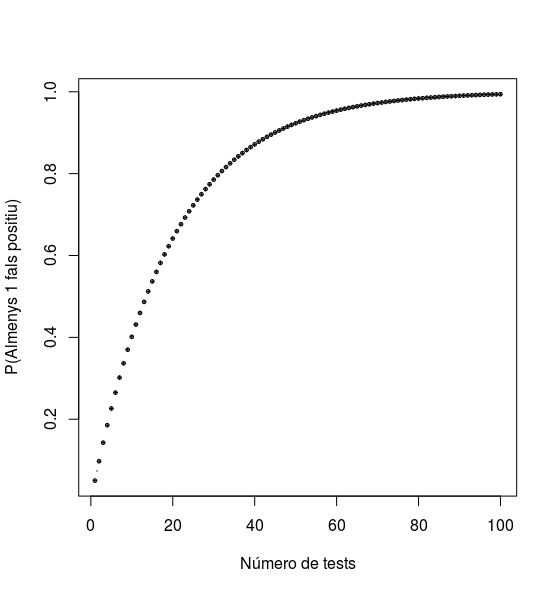
\includegraphics[scale=0.5]{FalsPositiu.png}
\captionof{figure}{Gràfic contraposant el nombre de tests amb la probabilitat d'obtenir almenys 1 fals positiu. S'observa un increment en la probabilitat quan augmenta el nombre de tests.}
\end{center}
En el nostre estudi es important tenir clar aquest problema, ja que si tenim molts gens, i no apliquem una correcció, podem caure en l'error d'afirmar que un gen s'expressa diferencialment quan realment no ho fa.
\subsubsection{Ratio falsos positius (\emph{False discovery Rate (FDR)})}
\label{2.2.1}
%http://www.gs.washington.edu/academics/courses/akey/56008/lecture/lecture10.pdf
%https://rpubs.com/Joaquin_AR/236898
Existeixen molts mètodes per corregir el problema de la multiplicitat de contrastos. El més simple és el mètode de Bonferroni, on cada p-valor es multiplica pel nombre de tests realitzats (acotant la probabilitat màxima a 1). És un mètode molt conservador i no és el més indicat per al nostre cas d'estudi.
Per a escenaris de \textit{large-scale multiple testing} com els estudis de genòmica, els quals es realitzen milers de test de forma simultània, el resultat dels mètodes clàssics de correcció (Bonferroni, Tukey, etc.) és massa conservador i impedeix que es detectin diferències reals. Una alternativa és controlar el \emph{FDR}.
\\

El  \emph{FDR} es defineix com la proporció esperada de falsos positius d'entre tots els tests considerats com significatius. L'objectiu de controlar el \emph{FDR} es establir un límit de significació per a un conjunt de tests tal que, d'entre tots els tests considerats com significatius, la proporció de falsos positius no superin un determinat valor.
Un altre avantatge afegit és la seva fàcil interpretació, per exemple, si un estudi publica resultats estadísticament significatius per a un $FDR$ del 10$\%$, el lector té la seguretat que, com a màxim, un 10$\%$ dels resultats considerats com a significatius poden ser realment falsos positius.
\\
La primera aproximació per controlar el \emph{FDR} va ser descrita per Benjamini $\&$ Hochberg en 1995. D'acord amb la seva publicació \cite{fdr}, si es desitja controlar que en un estudi amb $n$ comparacions el \emph{FDR} no superi un percentatge $d$ hem de:

\begin{itemize}
\item Ordenar els $n$ tests de menor a major p-valor ($p_{1}$,$p_{2}$,..., $p_n$).
\item Es defineix $k$ com l'última posició per la qual es compleix que $p_i \leq d\frac{i}{n}$.
\item Es consideren significatius tots els p-valors fins a la posició $k$ ($p_{1}$,$p_{2}$,..., $p_k$).

\end{itemize}

El mètode proposat per Benjamini $\&$ Hochberg assumeix a l'hora d'estimar el nombre d'hipòtesis nul·les erròniament considerades falses, que totes les hipòtesis nul·les són certes. Com a conseqüència, l'estimació del \emph{FDR} està inflada i és un mètode conservador. Per poder veure l'afectació d'utilitzar un mètode com Bonferroni o utilitzar el métode Benjamini $\&$ Hochberg, tenim la següent taula d'exemple:
\\
\begin{table}[ht]
\centering
\begin{tabular}{rrrr}
\hline
& P-valor & Bonferroni & Benjamini$\&$Hochberg \\
\hline
1 & 0.0010 & 0.0550 & 0.0037 \\
2 & 0.0020 & 0.11 & 0.0069 \\
3 & 1 & 1 & 1 \\
4 & 0.0010 & 0.0550 & 0.0037 \\
5 & 0.0010 & 0.0550 & 0.0037 \\
6 & 0.0010 & 0.0550 & 0.0037 \\
7 & 0.25 & 1 & 0.3929 \\
8 & 0.48 & 1 & 0.6286 \\
9 & 0.09 & 1 & 0.1650 \\
10 & 0.51 & 1 & 0.6523 \\
\hline
\end{tabular}
\caption{La primera columna de la taula conté els p-valors, sense corregir ni ordenar. La segona conté els p-valors amb la correcció de Bonferroni i la tercera el \emph{FDR} de Benjamini$\&$Hochberg, per a un total de 55 p-valors (Encara que només es mostren els 10 primers). Bonferroni és un mètode molt més conservador i cap p-valor és significatiu (dels 55 p-valors, 0 són significatius). En canvi, amb el mètode de Benjamini$\&$Hochberg, del total de p-valors, hi ha 26 significatius (en aquest cas hem fixat un $\alpha=0.05$ i un \emph{FDR}$=0.05$) }
\end{table}

A l'hora de decidir quin tipus de correcció aplicar, és important utilitzar un mètode adequat per tal d'obtenir resultats més acurats. Els mètodes que només depenen del nombre de tests no són els més potents com hem vist anteriorment.
\newpage
\subsection{Comparacions múltiples}
Un cop realitzat l'anàlisi de la variància i si aquest confirma l'existencia de diferències significatives entre els grups o tractaments, és convenient investigar quines mitjanes són diferents. El conjunt de tècniques que tracten aquest problema es denominen \textit{contrastos per comparacions múltiples}.
\\

\subsubsection{Métode de Tukey (\textit{honestly-significant-difference})}
%http://www.ugr.es/~bioestad/guiaspss/practica7/ArchivosAdjuntos/ComparacionesMultiples.pdf
%http://www2.hawaii.edu/~taylor/z631/multcomp.pdf
Recordem que quan el nombre de possibles comparacions és elevat, per a un nivell de significació $\alpha$ donat, pot conduir a una inflació de l'error de tipus I, com també hem vist quan parlàvem de multiplicitat de contrastos.
\\
Per identificar quins tractaments són significativament diferents entre ells i corregir el problema de la inflació de l'error de tipus I, hem utilitzat el mètode de Tukey i les seves hipòtesis són:

\begin{equation*}
H_{0}: \mu_i = \mu_j \text{ per a cada parella de mitjanes }  i \neq j
\end{equation*}
\vspace{-0.5cm}
\begin{equation*}
H_{1}: \mu_i \neq \mu_j \text{ almenys una parella de mitjanes }  i \neq j
\end{equation*}
\\
Aquest contrast es basa en la distribució del rang estudentitzat, que es defineix a partir del nombre de grups a comparar i dels graus de llibertat de l'estimador de la variància. Aquests tipus de procediments, permeten superar les dificultats que hi ha quan augmentem el nombre de grups a comparar i no podem controlar els falsos positius. En general, són mètodes conservadors, es a dir, la probabilitat real de rebutjar la hipòtesi nul·la quan és certa és menor que el nivell de significació $\alpha$ fixat.
\\

Per definir el rang estudentitzat, suposem que disposem de $k$ observacions independents $y_1,y_2,...,y_k$ d'una distribució Normal amb mitjana $\mu$ i variància $\sigma^2$. Suposem també que disposem d'un estimador $S^2$ de $\sigma^2$ que té $v$ graus de lliberat i és independent de les $y_i$. Definim $R$ com el rang d'aquest conjunt d'observacions,
\begin{equation*}
R = max(y_i) - min(y_i)
\end{equation*}
Sota aquestes condicions, es defineix el rang estudentitzat com el quocient,
\begin{equation*}
\frac{max(y_i) - min(y_i)}{S} = \frac{R}{S}
\end{equation*}
que es denota com $q_{k,v}$. Aquest estadístic segueix una distribució que depèn dels paràmetres $k$ i $v$, coneguda com la distribució del rang estudentitzat.
\\

L'estadístic de contrast que utilitza el test de Tukey queda definit com:
\begin{equation*}
Q_{I,n-I} = q_{I,n-I}(\alpha)\sqrt{\frac{MSE}{n}} ,
\end{equation*}
on $q_{I,n-I}$ és la quantila teòrica,
\begin{equation*}
q_{I,n-I}(\alpha) = \frac{\bar{X}_j - \bar{X}_k}{\sqrt{\frac{\hat{S}^2}{n}}}
\end{equation*}
$\hat{X}_j$ i $\hat{X}_k$ són la mitjana del grup $j$ i $k$, respectivament, i $\hat{X}_j > \hat{X}_k$. $\hat{S}^2$ és l'estimació de la variància del error o residual; i $n$ és la grandària mostral per a tots els grups; on $I$ i $n-I$ són els graus de llibertat de la distribució del rang estudentitzat ($I$ correspon al nombre de nivells que té el factor, $n$ correspon a la grandària mostral).En el cas de tenir grandàries mostrals diferents entre els nivells del factor, hem d'utilitzar un altre $n$ (mitjana harmònica):
\begin{equation*}
n_h = \frac{t}{\sum_{i=1}^{t}\frac{1}{n_i}}
\end{equation*}
\\

La diferència entre mitjanes serà significativa amb un nivell de significació $\alpha$ si
\begin{equation*}
|\bar{X}_j - \bar{X}_k |> HSD
\end{equation*}
on $HSD=Q_{I,n-I}$.

L'interval de confian\c{c}a per a la diferència de mitjanes el definim com:
\begin{equation*}
IC(\mu_j - \mu_k)_{(1-\alpha)}= (\bar{X}_j - \bar{X}_k) \pm q_{I,n-I,1-\alpha}\sqrt{\frac{MSE}{n}}
\end{equation*}
Si l'interval de la diferència inclou el 0, no rebutjem la hipòtesi nul·la del test i per tant, no hi ha diferències entre $\mu_j$ i $\mu_k$.
\subsection{Mètodes descriptius visuals}
\label{2.4}
%http://mural.uv.es/rata3/PECS/Genomica%20Funcional%20y%20Analisis%20de%20Microarrays%20PEC2.pdf
A l'hora de crear el protocol d'anàlisi teníem la necessitat de descriure el comportament de l'expressió dels gens segons el tractament i tenint en compte la funcionalitat de la família del gen. Una manera de veure aquests patrons era amb l'ús de tècniques visuals, que tenen una base matemàtica que explicarem en els següents apartats.
\subsubsection{Heatmap}
\label{2.4.1}
%http://wpd.ugr.es/~bioestad/guia-spss/practica-8/#8
%http://www.opiniomics.org/you-probably-dont-understand-heatmaps/
Un \textit{heatmap} (o mapa de calor) és una representació gràfica de dades on els valors individuals continguts en una matriu es representen com a colors.
\\

En mapes de calor, les dades es mostren en una quadrícula on cada fila representa un gen i cada columna representa una mostra o cas. El color i la intensitat de les caselles s'utilitzen per representar canvis en l'expressió gènica.
\\

L'exemple de la Figura 2 l'hem obtingut amb l'aplicatiu que hem creat:
\begin{center}
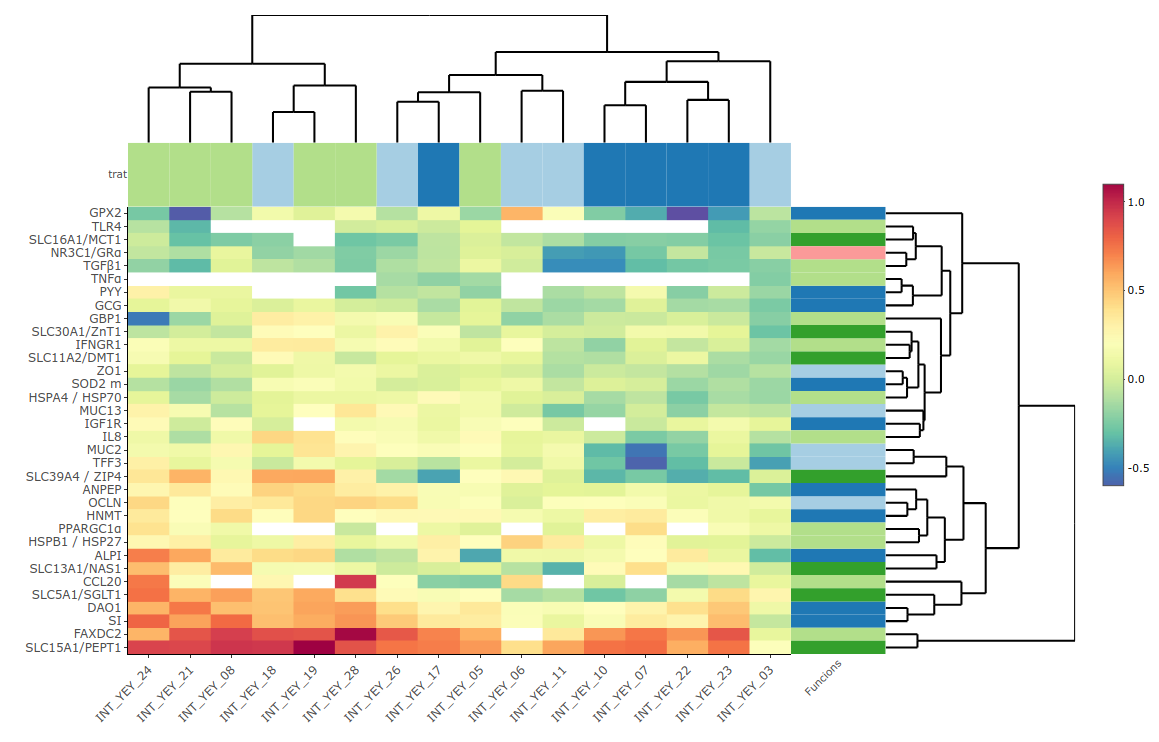
\includegraphics[scale=0.2]{heatmap.png}
\captionof{figure}{\texttt{Heatmap} generat a partir de 34 gens i 16 mostres. A les files trobem els gens i a les columnes les mostres.Veiem agrupacions (clústers) tant de gens com de mostres obtingudes mitjançant un algoritme jeràrquic. Per obtenir més informació, s'ha afegit variables alienes a la matriu d'expressions , concretament, a quin tractament correspon la mostra, i quina funció desenvolupa el gen.}
\end{center}

El mapa de calor també es pot combinar amb mètodes de \textit{clustering} que agrupen els gens i les mostres junts en funció de la similitud del seu patró d'expressió gènica. Això pot ser útil per identificar els gens que normalment s'expressen molt semblant i detectar patrons sota condicions o covariables establertes. El mètode implementat per la funció \texttt{heatmap}, utilitza l'anàlisi de clústers jeràrquics.
\\

En el cas dels mètodes jeràrquics les dades s'ordenen en nivells de manera que els nivells superiors contenen als inferiors. La jerarquia construïda permet obtenir també una partició de les dades en grups. S'utilitza la matriu de distàncies o similituds entre els elements de la matriu original de les dades.
\\

Els algoritmes \textit{jeràrquics} poden ser de dos tipus: De divisió i d'aglomeració.
\\

L'\textit{algoritme de divisió} assumeix que en un primer pas totes les dades conformen un sol conglomerat. Aquest clúster es va dividint successivament en conglomerats més petits d'acord a algun criteri seleccionat prèviament. El resultat d'aquest procediment es representa pel dendrograma.
\\

L'\textit{algoritme d'aglomeració} assumeix que cada observació inicialment és un conglomerat i en cada pas s'associen els conglomerats més similars fins a arribar a un sol clúster.
\\

La implementació \texttt{hclust} (\textit{hierarchical cluster analysis}) de \texttt{R} utilitza el \textit{Mètode de Ward} que calcula i actualitza a cada pas la dissimilaritat entre clústers, aquest mètode és d'aglomeració.
\\
\clearpage
\noindent\textbf{Mètode de Ward}
\\
%http://www.ugr.es/~gallardo/pdf/cluster-3.pdf

\noindent Ward va proposar que la pèrdua d'informació que es produeix en integrar els diferents individus en clústers pot mesurar-se a través de la suma total dels quadrats de les desviacions entre cada punt (individu) i la mitjana del clúster en el qual s'integra. Perquè el procés de clusterització resulti òptim, en el sentit que els grups formats no distorsionin les dades originals, proposava la següent estratègia:
\\

A cada pas de l'anàlisi, es considera la possibilitat de la unió de cada parell de grups i s'obta per la fusió d'aquells dos grups que menys incrementin la suma dels quadrats de les desviacions en unir-se.
\\

Definim:
\begin{itemize}
\item $x_{ij}^k$ com el valor de la $j$-èssima variable sobre l'$i$-èssim individu del $k$-èssim clúster, que té $n_k$ individus.
\item $m^k$ com el centroide del clúster $k$, amb components $m_{j}^k$.
\item $E_k$ com la suma de quadrats dels errors del clúster $k$, és a dir, la distancia euclídea al quadrat entre cada individu del cluster $k$ al seu centroide:
\begin{equation*}
E_k = \sum_{i=1}^{n_k}\sum_{j=1}^{p}(x_{ij}^k - m_{j}^k)^2
\end{equation*}
\item $E$ com la suma de quadrats dels errors per a tots els clústers, és a dir, si suposem $h$ clústers:
\begin{equation*}
E = \sum_{k=1}^{h} E_k
\end{equation*}
\end{itemize}
El procés comen\c{c}a amb $m$ clústers, cada clúster només té un sol individu, per tant, cada individu coincideix amb el centre del clúster i en aquest primer pas $E_k=0$, per a cada clúster i això fa que $E=0$. L'objectiu del mètode de Ward és trobar en cada etapa aquells dos clústers els quals la seva unió proporcioni el menor increment en la suma total d'errors $E$. Suposem que els clústers $C_p$ i $C_q$ s'uneixen resultant un nou clúster $C_t$, llavors definim l'increment de $E$ com,
\begin{equation*}
\bigtriangleup E_{pq} = E_t - E_p - E_q
\end{equation*}
el procés es repeteix fins a l'obtenció del dendrograma i l'agrupació dels individus en els diferents clústers. Un exemple aclaridor d'aquest procés iteratiu, amb dades reals, es pot trobar a l'annex \ref{annex:a}.
\newpage
\subsubsection{Anàlisi de components principals (ACP): gràfiques}
%http://www.knowledgeviz.com/pdf/UKC2009.pdf
%http://www.econ.upf.edu/~satorra/M/ComponentsPrincipals.pdf
L'anàlisi de components principals és una de les diferents maneres per analitzar l'estructura d'una matriu de correlacions donada. En aquest apartat definirem la teoria de l'anàlisi de components principals i la seva representació gràfica.
\\

\noindent\textbf{L'objectiu de l'ACP}\\
Donades $p$ variables $X_1,X_2, \ldots,X_p$ que suposarem centrades
(sovint també normalitzades amb variància igual a 1), volem
construir $p$ noves variables $Z_1,Z_2, \ldots,Z_p$, que anomenarem
compoents (les components principals seran cert subconjunt
d'aquestes) amb les següents condicions:
\begin{enumerate}
 \item Les noves variables han de ser combinació lineal de les
 variables originals.
 \item Les noves variables han de ser incorrelacionades.
 \item Les noves variables han de contenir la mateixa informaicó (variància
 total) que les originals, i estar ordenades de major a menor
 variància.
\end{enumerate}
El teorema que demostra l'existència i unicitat de les components, i
en dóna el procediment de càlcul és el següent:


\begin{theorem}
Les components  venen donades per la transformació lineal
$$Y =V^tX$$
on la matriu $V$ és la matriu ortogonal de vectors propis columna
donada per la descomposició espectral (Jordan) de $\Sigma$ - la
matriu de covariàncies de $X$ -, amb els vectors propis ordenats
segons el valor propi $\lambda_j$, de més gran a més petit. A més,
com que la descomposició espectral compleix
\begin{equation}
\Sigma=V\Lambda
V^t, \label{sig}
\end{equation}
amb $\Lambda$ la matriu diagonal de
valors propis. La descomposició (\ref{sig}) és equivalent a
\begin{equation}
\Lambda=V^t\Sigma V=\Sigma_Z.
\label{lam}
\end{equation}
\end{theorem}

De la igualtat (\ref{lam}) del teorema teorema es dedueix que les
components són incorrelacionades perquè tenen matriu de covariàncies
diagonal i estan ordenades de major a menor variancia. En particular
tenim que
$$Var (Z_j ) = \lambda_j,\quad\mbox{amb}\quad \lambda_1\geq\lambda_2\geq \ldots \geq \lambda_p.$$
De l'equació  (\ref{lam}), igualant les traces, tenim que:
\begin{equation}
 VT(Z):= \lambda_1+\lambda_2+\cdots + \lambda_p=\sigma_1^2 +\sigma_2^2+\cdots + \sigma_p^2=: VT(X)\ \label{pcv}
\end{equation}
on $VT$ indica la variància total. Aquesta igualtat (\ref{pcv})
s'anomena \emph{principi de conservació de la variància}.
\clearpage
De tot l'anterior, és lògic que s'escullin les $k$ primeres
components, si representen un percentatge ``prou important'' (70\%,
80\%, etc.,) de la variància total: $$
\frac{\lambda_1+\ldots+\lambda_k}{\lambda_1+\ldots+\lambda_p} \geq
0.7  \mbox{ (o bé 0.8, etc.)}
$$
Les $k$ primeres components, escollides segons aquest o un altre
criteri, s'anomenen \emph{components principals}.

Pel cas més habitual en que les variables inicials estan
estandarditzades (centrades i escalades), és a dir $\sigma_i^2=1$,
$\,\forall i$, es té que
$$
\lambda_1+\lambda_2+\cdots + \lambda_p=1.
$$



\subsubsection{Gràfica de les variables}
\label{2.4.3}
 Suposem variables centrades i escalades. La matriu $W=V\Lambda^{1/2}$
s'anomena matriu de pesos (\emph{loadings})  i dóna les coordenades
per expressar  les variables com a combinació lineal (o mitjana
ponderada) de les components (veure la gràfica de les variables, a
l'apartat següent). Si suposem que $k=2$, la variable original $X_i$
 es representa amb les coordenades $(w_{i1,w_i2})$, en forma de ``fletxa''. La igualtat
 (\ref{sig}) és equivalent a
 $$
 \Sigma=W^tW
 $$
 Pels termes diagonals, resulta:
 $$
 \sigma_i^2=1=w_{i1}^2+w_{i2}^2+\cdots+w_{ip}^2
 $$
Per tant, els coeficients $w_{ij}^2$, o cosinus quadrats, sumen 1 i,
si la variable està ben representada en dimensió $k=2$, es té que
$$
\mbox{long.vector}^2=w_{i1}^2+w_{i2}^2\approx 1
$$
i la fletxa d'aquesta variable s'apropa a la circumferència de radi
1.
\\

Si una variable quedés explicada en un $100\%$, la longitud del vector seria 1. Si, en canvi, quedés molt mal explicada, la longitud del vector corresponent seria propera a zero. Per tant, com més properes al cercle unitat estiguin les variables, més llargues seran les fletxes i millor quedaran representades. És a dir, menor serà la pèrdua d'informació que es produeix en substituir les variables originals per les components principals.
En aquest exemple, el gràfic ens mostra que les quatre variables queden molt ben
representades.
\\

``\textit{Els angles que formen dues fletxes entre sí, ens mostren la correlació existent entre les corresponents variables}''
\\

El cosinus de l'angle format pels dos vectors és proporcional a la seva correlació. Com
més petit sigui l'angle, més gran la correlació. Així, dues variables que quedin
representades en punts molt propers tindran vectors que formaran un angle proper a zero, fet que indica que tindran una correlació molt forta. En canvi, dues variables representades per punts molt separats i els vectors de les quals formin un angle proper a l'angle recte, seran pràcticament incorrelacionades.
\\

``\textit{Els sentits dels vectors indiquen el signe de la correlació existent entre les
corresponents variables}''
\\

Dos vectors que tinguin una mateixa direcció però sentits oposats tindran una correlació
molt forta en sentit negatiu. És a dir, valors elevats en una variable es corresponen amb
valors baixos en l'altra.
\\

``\textit{La posició de les variables en el gràfic mostra l'estructura de les dades i suggereix possibles interpretacions de les components principals}''
\\

El fet que hi hagi un grup de variables ben representades i en posicions properes en el
gràfic indica que totes elles estan molt relacionades entre sí i que ens subministren
bàsicament la mateixa informació. Quan apareixen varis grups de variables vol dir que hi
ha diferents aspectes descrits per la matriu de dades. També el fet que alguna variable quedi molt ben representada i que en el gràfic li correspongui un punt proper a un dels eixos de coordenades, ens està indicant que una de les dues primeres components principals està fortament correlacionada amb aquesta variable i, per tant, se li pot donar una interpretació similar.


%%% RESULTS
\clearpage
\section{Cas d'estudi}
El cas d'estudi consisteix en un disseny experimental fet amb porcins que han sigut alimentats amb diferents fonts de proteïnes (diverses combinacions de productes de soja, plasma animal i mucosa) a principis del deslletament. L'objectiu principal del estudi és avaluar la salut intestinal del porc poc després d'administrar les diferents dietes. A més, és vol veure si els tractaments tenen un efecte en el creixement del porc, i per tant, en la productivitat de l'empresa.
\subsection{Descripció de l'estudi}
L'estudi es defineix breument en els següents punts\\

\noindent\textbf{Objectiu de l'estudi}
\begin{itemize}
  \item Analitzar i comparar els diferents tractaments i com afecten a l'expressió dels gens.
  \item Trobar relacions entre la funcionalitat del gen i la seva expressió sota diferents tractaments.
\end{itemize}
\noindent\textbf{Disseny de l'estudi}\\
Estudi experimental amb una mostra total de 48 casos. És un un dels primers experiments realitzats pel \textit{SNiBA}, per tant, l'experiment es totalment exploratori i es podría definir com una prova per a futurs dissenys.
\noindent\textbf{Tractaments}
\begin{itemize}
  \item \textbf{T1}: Inclusió d'aliments de soja a la dieta.
  \item \textbf{T2}: Inclusió de plasma animal a la dieta.
  \item \textbf{T3}: Inclusió de $33\%$ de plasma animal i  $66\%$ de mucosa a la dieta.
  \item \textbf{T4}: Inclusió de $50\%$ de plasma animal i  $50\%$ de mucosa a la dieta.
\end{itemize}
\noindent\textbf{Variables explicatives}\\
La principal variable explicativa és:
\begin{itemize}
  \item Tractament
\end{itemize}
Les variables secundàries que també trobem a l'estudi:
\begin{enumerate}
  \item ID: nom del cas.
  \item Teixit: l'estudi es fa paral·lelament amb 2 tipus de teixits diferents, per tant, es farà un estudi amb cada teixit. (Dels 48 casos, queden 24 casos per teixit)
  \begin{itemize}
    \item Jejunum
    \item Ileum
  \end{itemize}
\end{enumerate}
\noindent\textbf{Variables genètiques}\\
Cada gen és una variable on es mesura l'abundancia de material genètic. Els gens han sigut escollits pels investigadors basant-se en les seves recerques i reben el nom de gens \textit{diana}. A l'annex \ref{annex:b} trobem una taula de tots els gens de l'estudi amb la seva funcionalitat dins de l'organisme.
\newpage
\noindent\textbf{Tractament de dades faltants}\\
El tractament dels NA’s és el següent:
\begin{enumerate}
\item S’eliminen aquelles files i columnes sense cap observació vàlida.
\item S’eliminen aquelles columnes (gens) que tinguin més del 50$\%$ de valors perduts en algun tractament.
\end{enumerate}
\noindent\textbf{Mètodes estadístics}\\
L'anàlisi estadístic ha sigut realitzat utilitzant \texttt{R} amb la versió 3.4.3.
\\

Per a tots els tests estadístics s'ha aplicat un nivell de significació del $5\%$ (P < 0.05). S'han realitzat correccions per multiplicitat de contrastos; \textit{Benjamini$\&$Hochberg} per l'ANOVA i \textit{Tukey} per les comparacions 2 a 2 entre tractaments.
\\

Tota la documentació, codi i \textit{outputs} han sigut emmagatzemats en un repositori públic a la plataforma \textit{GitHub}.\\
\noindent\textbf{Tractament de les dades}\\
Les dades han sigut validades abans de l'anàlisi, qualsevol inconsistencia en el format de les dades ha sigut eliminat o canviat. Més endavant s'expliquen quins criteris de l'estructura de la base de dades són els adequats perquè sigui funcional a l'aplicatiu.
\\

A més, hem aplicat una tranformació logarítmica als valors d'expressió gènica per a cada gen, amb l'objectiu de treballar amb una distribució normal i poder aplicar els mètodes estadístics descrits anteriorment.
\begin{center}
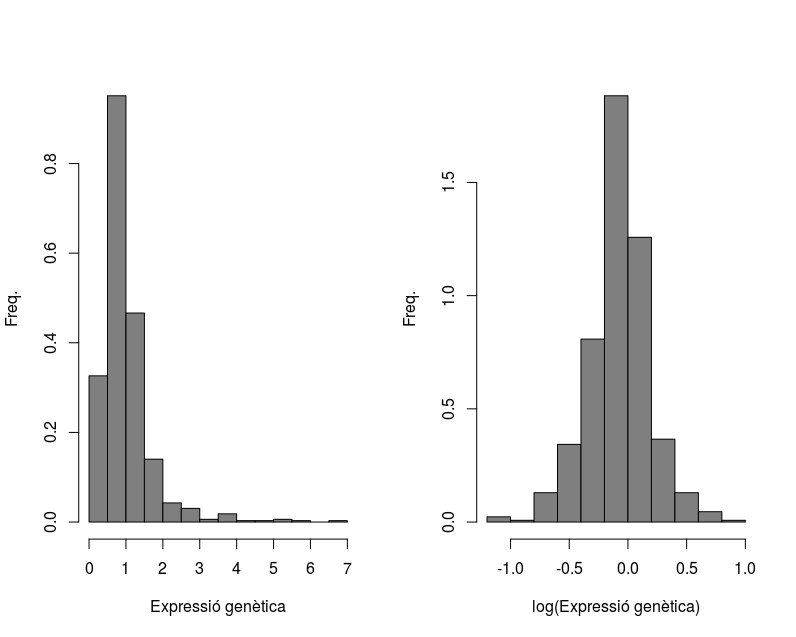
\includegraphics[scale=0.45]{logsdades.png}
\captionof{figure}{(1) El gràfic de l'esquerra mostra les dades sense cap tipus de transformació.(2) El gràfic de la dreta mostra les dades amb una transformació logarítmica.}
\end{center}
\clearpage
\subsection{Resultats}
Degut al disseny de l'estudi, s'analitzen paral·lelament 2 tipus de teixits, \textit{Ilenum} i \textit{Jejunum}. L'anàlisi que es duu a terme consta d'una primera part on s'examinen quins gens s'expressen diferencialment en cada teixit sota els 4 tractaments, i es determinen quins tractaments són diferents entre ells per a cada gen. Després hi ha una segona part més desciptiva on s'analitzen els patrons trobats en els mètodes visuals.
\subsubsection{Anàlisi de la variància (ANOVA)}
Amb l'objectiu de trobar quins gens s'expressen diferencialment sota els diferents tractaments s'ha aplicat l'anàlisi de la variancia per a cada teixit:
\begin{table}[ht]
\centering
\begin{tabular}{rlrrc}
    \toprule
{\textbf{Nom del gen}} & {\textbf{Funció del gen }} & {\textbf{Estadístic F}} & {\textbf{P-valor}} & {\textbf{P-valor (Benjamini$\&$Hochberg)}} \\
  \midrule
{\textcolor{gray}{TFF3}} & Barrier Function & 5.2927 & 0.0086 & $0.0603^{*}$ \\
  {\textcolor{gray}{OCLN}} & Barrier Function & 1.2861 & 0.3094 & 0.4572 \\
  {\textcolor{gray}{ZO1}} & Barrier Function & 0.9128 & 0.4544 & 0.5979 \\
  {\textcolor{gray}{MUC2}} & Barrier Function & 7.2461 & 0.0022 & $0.0272^{***}$ \\
  {\textcolor{gray}{MUC13}} & Barrier Function & 2.1769 & 0.1261 & 0.2425 \\
  {\textcolor{gray}{SI}} & Enzymed/Hormone & 3.1867 & 0.0488 & 0.1525 \\
  {\textcolor{gray}{DAO1}} & Enzymed/Hormone & 1.2813 & 0.3109 & 0.4572 \\
  {\textcolor{gray}{HNMT}} & Enzymed/Hormone & 0.5736 & 0.6396 & 0.6953 \\
  {\textcolor{gray}{ANPEP}} & Enzymed/Hormone & 1.9658 & 0.1553 & 0.2773 \\
  {\textcolor{gray}{GCG}} & Enzymed/Hormone & 1.1972 & 0.3390 & 0.4709 \\
  {\textcolor{gray}{IGF1R}} & Enzymed/Hormone &  &  &  \\
  {\textcolor{gray}{GPX2}} & Enzymed/Hormone & 10.5231 & 0.0003 & $0.0079^{***}$\\
  {\textcolor{gray}{SOD2m}} & Enzymed/Hormone & 3.3427 & 0.0424 & 0.1516 \\
  {\textcolor{gray}{ALPI}} & Enzymed/Hormone & 2.1929 & 0.1241 & 0.2425 \\
  {\textcolor{gray}{TNF$\alpha$}} & Inmune Response &  &  &  \\
  {\textcolor{gray}{TGF$\beta_1$}} & Inmune Response & 1.7353 & 0.1956 & 0.3260 \\
  {\textcolor{gray}{CCL20}} & Inmune Response &  &  &  \\
  {\textcolor{gray}{IFNGR1}} & Inmune Response & 4.5897 & 0.0148 & $0.0741^{*}$ \\
  {\textcolor{gray}{HSPB1.HSP27}} & Inmune Response & 0.8298 & 0.4947 & 0.6184 \\
  {\textcolor{gray}{HSPA4.HSP70}} & Inmune Response & 0.6819 & 0.5745 & 0.6529 \\
  {\textcolor{gray}{FAXDC2}} & Inmune Response &  &  &  \\
  {\textcolor{gray}{GBP1}} & Inmune Response & 0.6991 & 0.5647 & 0.6529 \\
  {\textcolor{gray}{IL8}} & Inmune Response & 5.1389 & 0.0096 & 0.0603 \\
  {\textcolor{gray}{SLC5A1.SGLT1}} & Nutrient Transport& 2.5431 & 0.0886 & 0.2013 \\
  {\textcolor{gray}{SLC16A1.MCT1}} & Nutrient Transport & 0.1985 & 0.8961 & 0.9334 \\
  {\textcolor{gray}{SLC15A1.PEPT1}} & Nutrient Transport &  &  &  \\
  {\textcolor{gray}{SLC13A1.NAS1}} & Nutrient Transport & 2.8547 & 0.0661 & 0.1652 \\
  {\textcolor{gray}{SLC11A2.DMT1}} & Nutrient Transport &  &  &  \\
  {\textcolor{gray}{SLC30A1.ZnT1}} & Nutrient Transport & 4.2445 & 0.0196 & $0.0818^{*}$ \\
  {\textcolor{gray}{SLC39A4.ZIP4}} & Nutrient Transport & 3.0217 & 0.0567 & 0.1575 \\
  {\textcolor{gray}{NR3C1.Gr$\alpha$}} & Stress & 0.0308 & 0.9925 & 0.9925 \\
   \bottomrule
\end{tabular}
\caption{P-valors de l'ANOVA entre tractaments pel teixit \textbf{Ileum}. Els p-valors per sota de 0.05 queden marcats amb $^{***}$ i per sota de 0.1 amb $^{*}$.}
\end{table}

\noindent El nivell de significació és $\alpha$=0.05, però degut al conjunt de tests realitzats s'aplica una correcció (\textit{Benjamini $\&$ Hochberg}). Per tant, només s'haurien de considerar significatius del conjunt experimental aquells tests en els que el p-valor de \textit{Benjamini $\&$ Hochberg} estigui per sota de determinat llindar, en aquest cas hem fixat un nivell de significació del 5$\%$, encara que en aquests tipus d'experiments poden arribar al $10\%$. Observem que hi ha gens sense cap p-valor, això es degut a que després de fer el tractament de dades faltants (descrit a l'apartat anterior) encara hi ha NA's, per tant, l'anàlisi de la variància no contempla aquests gens.
\clearpage
%Jejunum
\begin{table}[ht]
\centering
\begin{tabular}{rlrrc}
  \toprule
 {\textbf{Nom del gen}} & {\textbf{Funció del gen }} & {\textbf{Estadístic F}} & {\textbf{P-valor}} & {\textbf{P-valor (Benjamini$\&$Hochberg)}} \\
  \midrule
{\textcolor{gray}{TFF3}} & Barrier Function & 5.2048 & 0.0099 & $0.0635^{*}$  \\
  {\textcolor{gray}{OCLN}} & Barrier Function & 3.7353 & 0.0314 & $0.0919^{*}$  \\
  {\textcolor{gray}{ZO1}} & Barrier Function & 2.4161 & 0.1020 & 0.1962 \\
  {\textcolor{gray}{MUC2}} & Barrier Function & 5.0794 & 0.0108 & $0.0635^{*}$  \\
  {\textcolor{gray}{MUC13}} & Barrier Function & 2.1372 & 0.1332 & 0.2220 \\
  {\textcolor{gray}{SI}} & Enzymed/Hormone & 3.6748 & 0.0331 & $0.0919^{*}$  \\
  {\textcolor{gray}{DAO1}} & Enzymed/Hormone & 4.8678 & 0.0127 & $0.0635^{*}$  \\
  {\textcolor{gray}{HNMT}} & Enzymed/Hormone & 4.5122 & 0.0167 & $0.0697^{*}$  \\
  {\textcolor{gray}{ANPEP}} & Enzymed/Hormone & 2.3119 & 0.1126 & 0.2011 \\
  {\textcolor{gray}{GCG}} & Enzymed/Hormone & 6.6996 & 0.0035 & $0.0433^{***}$ \\
  {\textcolor{gray}{IGF1R}} & Enzymed/Hormone &  &  &  \\
  {\textcolor{gray}{PYY}} & Enzymed/Hormone &  &  &  \\
  {\textcolor{gray}{GPX2}} & Enzymed/Hormone &  &  &  \\
  {\textcolor{gray}{SOD2m}} & Enzymed/Hormone & 1.4329 & 0.2680 & 0.3526 \\
  {\textcolor{gray}{ALPI}} & Enzymed/Hormone & 1.0417 & 0.3994 & 0.4755 \\
  {\textcolor{gray}{TLR4}} & Inmune Response &  &  &  \\
  {\textcolor{gray}{TGF$\beta1$}} & Inmune Response & 1.7069 & 0.2034 & 0.3178 \\
  {\textcolor{gray}{CCL20}} & Inmune Response &  &  &  \\
  {\textcolor{gray}{IFNGR1}} & Inmune Response & 1.5036 & 0.2495 & 0.3526 \\
  {\textcolor{gray}{HSPB1.HSP27}} & Inmune Response & 0.3366 & 0.7991 & 0.8324 \\
  {\textcolor{gray}{HSPA4.HSP70}} & Inmune Response & 0.8326 & 0.4943 & 0.5617 \\
  {\textcolor{gray}{FAXDC2}} & Inmune Response &  &  &  \\
  {\textcolor{gray}{GBP1}} & Inmune Response & 0.0084 & 0.9989 & 0.9989 \\
  {\textcolor{gray}{IL8}} & Inmune Response & 2.5729 & 0.0881 & 0.1835 \\
  {\textcolor{gray}{SLC5A1.SGLT1}} & Nutrient Transport & 4.1519 & 0.0223 & $0.0796^{*}$  \\
  {\textcolor{gray}{SLC16A1.MCT1}} & Nutrient Transport &  &  &  \\
  {\textcolor{gray}{SLC15A1.PEPT1}} & Nutrient Transport & 2.9677 & 0.0613 & 0.1394 \\
  {\textcolor{gray}{SLC13A1.NAS1}} & Nutrient Transport & 3.5486 & 0.0368 & $0.0921^{*}$  \\
  {\textcolor{gray}{SLC11A2.DMT1}} & Nutrient Transport & 1.3570 & 0.2895 & 0.3618 \\
  {\textcolor{gray}{SLC30A1.ZnT1}} & Nutrient Transport & 0.4630 & 0.7118 & 0.7737 \\
  {\textcolor{gray}{SLC39A4.ZIP4}} & Nutrient Transport & 19.3772 & 0.0000 & $0.0003^{***}$ \\
  {\textcolor{gray}{NR3C1.Gr$\alpha$}} & Stress & 1.4606 & 0.2606 & 0.3526 \\
   \bottomrule
\end{tabular}
\caption{P-valors de l'ANOVA entre tractaments pel teixit \textbf{Jejunum}. Els p-valors per sota de 0.05 queden marcats amb $^{***}$ i per sota de 0.1 amb $^{*}$.}
\end{table}
\noindent\textbf{Ileum}\\
\\
Un cop fet l'ANOVA i la corresponent correcció per multiplicitat de contrastos (FDR), s'han trobat 2 gens amb una expressió diferencial (p-valor < 0.05), \textit{MUC2} i \textit{GPX2}. Anomenarem quasi significatius aquells gens que es troben entre $0.5 <$ p-valor $\leq 0.1$. Els gens quasi significatius són 3; \textit{TFF3}, \textit{IFNGR1} i \textit{SLC30A1.ZnT}. Podem trobar aquests resultats a la \textit{Taula 2}.\\
\\
\noindent\textbf{Jejunum}\\
\\
Un cop fet l'ANOVA i la corresponent correcció per multiplicitat de contrastos (FDR), s'han trobat 2 gens amb una expressió diferencial (p-valor < 0.05), \textit{GCG} i \textit{SLC39A4.ZIP4} Els gens quasi significatius són 8; \textit{TFF3}, \textit{OCLN}, \textit{MUC2}, \textit{SI}, \textit{DAO1}, \textit{HNMT}, \textit{SLC5A1.SGLT1} i \textit{SLC13A1.NAS1}. Podem trobar aquests resultats a la \textit{Taula 3}.\\

\clearpage
\subsubsection{Comparacions múltiples 2 a 2}
Un cop identificats els gens que han manifestat una expressió diferencial hem aplicat comparacions 2 a 2 amb l'objectiu de veure quins tractaments són diferents entre si. L'anàlisi esta fet per a cada teixit i el mètode utilitzat per corregir la multiplicitat de contrastos ha sigut el mètode de Tukey.
\begin{table}[ht]
\centering
\scalebox{0.75}{
\begin{tabular}{rrrrrrr}
  \toprule
 & {\textbf{2-1}} & {\textbf{3-1}} & {\textbf{4-1}} & {\textbf{3-2}} & {\textbf{4-2}} & {\textbf{4-3}} \\
  \midrule
{\textcolor{gray}{TFF3}} &  &  & 0.0044 &  &  &  \\
  {\textcolor{gray}{MUC2}} & 0.0399 &  & 0.0023 &  &  & 0.0243 \\
  {\textcolor{gray}{GPX2}} & 0.0028 &  & 0.0632 & 0.0006 &  & 0.0147 \\
  {\textcolor{gray}{IFNGR1}} &  & 0.0625 & 0.0160 &  &  &  \\
  {\textcolor{gray}{IL8}} & 0.0203 &  & 0.0329 &  &  &  \\
  {\textcolor{gray}{SLC30A1.ZnT1}} &  & 0.0984 &  & 0.0249 &  &  \\
   \bottomrule
\end{tabular}
}
\caption{Dels gens significatius per al teixit \textbf{Ilenum}, s'apliquen comparacions 2 a 2 Gene-Tractament. A la taula només es mostren aquells p-valors quasi significatius o significatius.}
\end{table}

Podem destacar que gairebé tots els gens que surten signficatius presenten diferències estadísticament significatives entre el tractament 4 i el tractament 1. De la mateixa manera, observem que la comparació entre el tractament 4-2 no indica cap diferència significativa.
\begin{center}
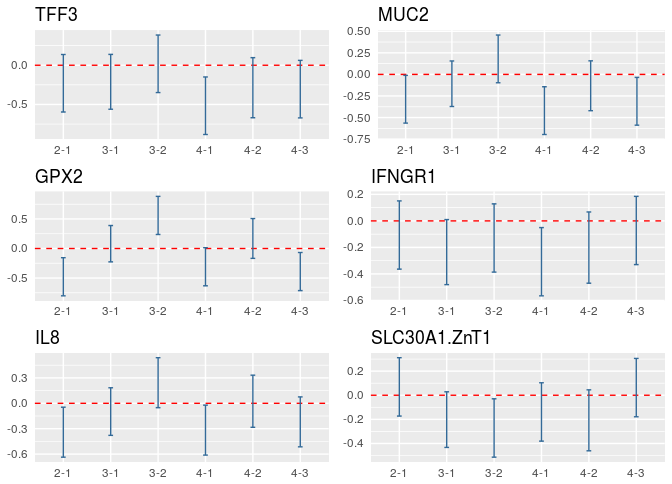
\includegraphics[scale=0.45]{IleumTukey.png}
\captionof{figure}{Intervals de confian\c{c}a del $95\%$ per a la diferència de mitjanes per a cada comparació i per a cada gen del teixit \textbf{Ilenum}. Els intervals que no contenen el 0, es mostren com comparacions estadísticament significatives.}
\end{center}
En el teixit \textit{Jejunum}, podem veure que cap gen presenta diferencies significatives entre el tractament 4 i 3. Les comparacions que presenten més diferencies són 3-2 i 4-2, encara que no és presenta un patró tan clar com en el teixit Ilenum.
\begin{table}[ht]
\centering
\scalebox{0.75}{
\begin{tabular}{rrrrrrr}
  \toprule
 & {\textbf{2-1}} & {\textbf{3-1}} & {\textbf{4-1}} & {\textbf{3-2}} & {\textbf{4-2}} & {\textbf{4-3}} \\
  \midrule
{\textcolor{gray}{TFF3}} &  &  &  & 0.0512 & 0.0074 &  \\
  {\textcolor{gray}{OCLN}} &  &  &  & 0.0510 & 0.0713 &  \\
  {\textcolor{gray}{MUC2}} &  &  &  & 0.0357 & 0.0098 &  \\
  {\textcolor{gray}{SI}} &  &  & 0.0283 &  &  &  \\
  {\textcolor{gray}{DAO1}} &  & 0.0422 & 0.0368 &  &  &  \\
  {\textcolor{gray}{HNMT}} &  & 0.0211 & 0.0357 &  &  &  \\
  {\textcolor{gray}{GCG}} &  & 0.0896 & 0.0142 & 0.0662 & 0.0100 &  \\
  {\textcolor{gray}{SLC5A1.SGLT1}} &  &  &  & 0.0842 & 0.0410 &  \\
  {\textcolor{gray}{SLC13A1.NAS1}} &  &  & 0.0286 &  &  &  \\
  {\textcolor{gray}{SLC39A4.ZIP4}} & 0.0015 &  &  & 0.0001 & 0.0000 &  \\
   \bottomrule
\end{tabular}
}
\caption{Dels gens significatius per al teixit \textbf{Jejunum}, s'apliquen comparacions 2 a 2 Gene-Tractament. A la taula només es mostren aquells p-valors quasi significatius o significatius.}
\end{table}

\begin{center}
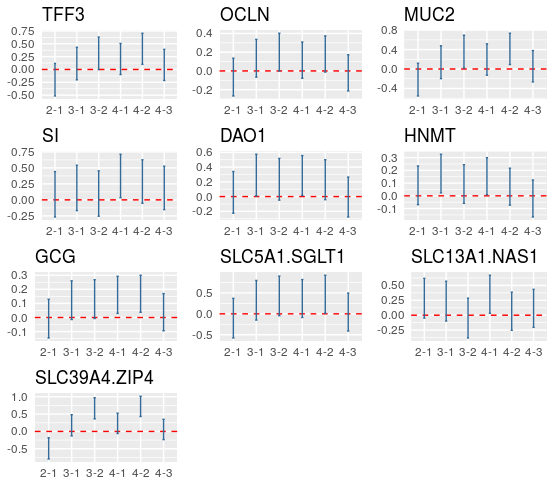
\includegraphics[scale=0.5]{TukeyJeju.png}
\captionof{figure}{Intervals de confian\c{c}a del $95\%$ per a la diferència de mitjanes per a cada comparació i per a cada gen del teixit \textbf{Jejunum}. Els intervals que no contenen el 0, es mostren com comparacions estadísticament significatives.}
\end{center}
\subsubsection{Mètodes visuals}
Els següents gràfics del protocol ens poden ajudar a trobar relacions i agrupacions entre els tractaments i els gens. El primer mètode analitzat ha sigut el ACP per a cada teixit:
\begin{center}
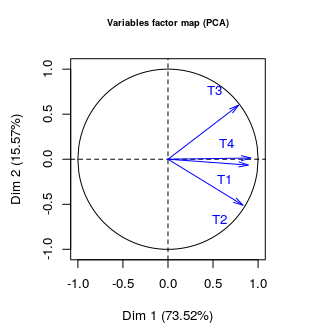
\includegraphics[scale=0.4]{biploti.png}
\captionof{figure}{Representació gràfica de l'ACP de les mitjanes per cada gene-tractament del teixit \textbf{Ilenum}.}
\end{center}
Amb aquest teixit podem observar una correlació alta entre la mitjana del tractament 4 i la mitjana del tractament 1. En canvi, trobem correlacions més febles entre el tractament 4 i els tractaments restants. L'angle entre el tractament 2 i el tractament 3, ens indica una correlació casi nul·la.
\begin{center}
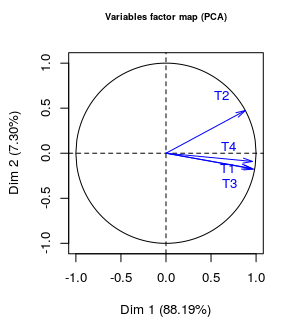
\includegraphics[scale=0.4]{biplotj.png}
\captionof{figure}{Representació gràfica de l'ACP de les mitjanes per cada gene-tractament del teixit \textbf{Jejunum}.}
\end{center}
En aquest cas trobem correlacions altes entre els tractaments 1, 3 i 4. En canvi el tractament 2, sembla tenir una correlació més feble amb els altres tractaments. Recordem que per calcular el coeficient de correlació en aquest gràfic, només necesitem l'angle que formen els dos vectors, suposem que l'angle entre T4 i T2 és de 45 graus:
\begin{equation*}
r(T4,T2)= cos(angle_{(T4,T2)})= cos(\frac{\pi}{4})= 0.7071
\end{equation*}
El següent gràfic mostra les mitjanes de cada gen per tractaments, d'aquesta manera es poden observar les diferències que observavem a l'ANOVA i a les comparacions 2 a 2.
\begin{center}
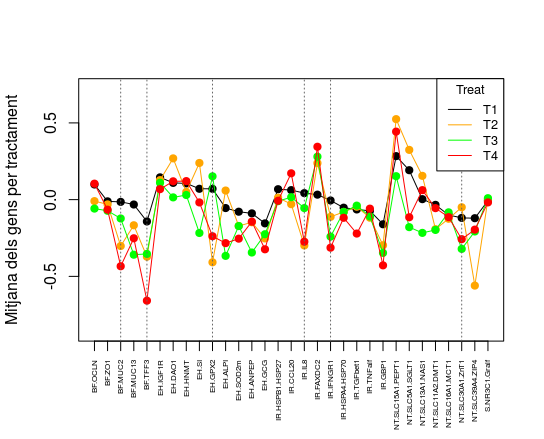
\includegraphics[scale=0.6]{lineploti.png}
\captionof{figure}{Mitjana dels gens per tractament, teixit \textbf{Ilenum}. El gràfic esta ordenat per família gènica primer i dins de la familia per el tractament 1 de forma decreixent. El nom de cada gen esta acompanyat de la seva funció dins de l'organisme, com per exemple, \textit{BF.OCLN} = funció del gen: \textit{Barrer Function}, nom del gen: \textit{OCLN}}
\end{center}
\begin{center}
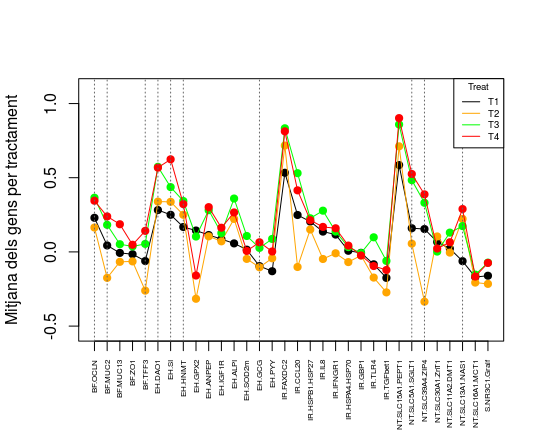
\includegraphics[scale=0.6]{lineplotj.png}
\captionof{figure}{Mitjana dels gens per tractament, teixit \textbf{Jejunum}. El gràfic esta ordenat per família gènica primer i dins de la familia per el tractament 1 de forma decreixent.}
\end{center}
Un fet imporant a destacar en el gràfic del texit \textbf{Jejunum}, és el gran número de gens significatius que tenen una funció barrera o protectora (BF) dins del organisme.\\

Per últim, es presenten els \textit{heatmap} per a cada teixit:
\begin{center}
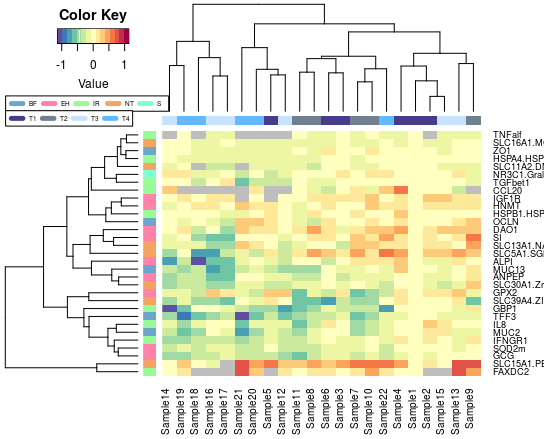
\includegraphics[scale=0.6]{heatmapi.png}
\captionof{figure}{Heatmap del teixit \textbf{Ilenum}.}
\end{center}
\begin{center}
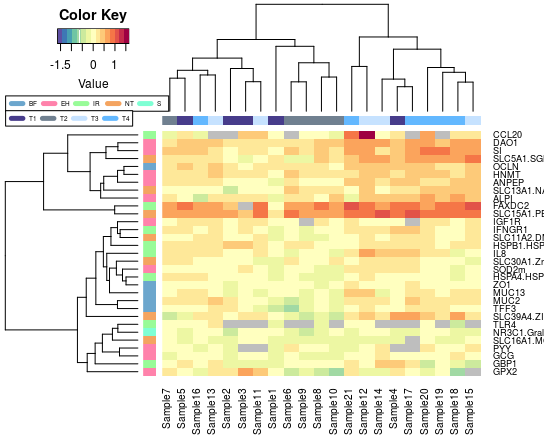
\includegraphics[scale=0.6]{heatmapj.png}
\captionof{figure}{Heatmap del teixit \textbf{Jejunum}.}
\end{center}

Les conclusions d'aquest apartat queden incloses en les conclusions finals del cas d'estudi.
\clearpage
\subsection{Conclusions (cas d'estudi)}

Un cop realitzat l'anàlisi per mitjà del protocol que hem desenvolupat, es l'hora de les conclusions. Recordem que és un estudi eminentment exploratori (en el sentit de que és un prototip o protocol d'actuació, sense gaires precedents en l'àmbit de la producció animal). Per tant, l'equip estadístic
ha tingut un paper clau en definir les hipotesis i criteris estadístics que creiem més importants. Aquests criteris pretenen ajudar a que els investigadors interpretin resultats presents o futurs.
\\

Els primers apartats del protocol consisteixen  en l'anàlisi separada per a cada gen fixat, però amb correcció FDR, atès que les anàlisis són simultànies. La primera hipòtesi de recerca que ens plantegem és:
\\

\textit{En algun gen (i quin o quins) hi ha diferències significatives en els nivells d'expressió entre tractaments?}
\\

Per al teixit \textit{Ilenum}, d'un total de 31 gens, s'han trobat 2 gens amb una expressió diferencial significativa (p-valor(Benjamini $\&$ Hochberg) $\leq$ 0.05), \textit{MUC2} i \textit{GPX2}. Anomenarem quasi significatius aquells gens que es troben entre $0.5 $ p-valor $\leq 0.1$. Els gens quasi significatius són 3: \textit{TFF3}, \textit{IFNGR1} i \textit{SLC30A1.ZnT}. Podem trobar aquests resultats a la \textit{Taula 2}.
\\

Per al teixit \textit{Jejunum}, d'un total de 32 gens, s'han trobat 2 gens amb una expressió diferencial (p-valor(Benjamini $\&$ Hochberg) $\leq$ 0.05), \textit{SLC39A4.ZIP4} i \textit{GCG}. Els gens quasi significatius són 8: \textit{TFF3}, \textit{OCLN}, \textit{MUC2}, \textit{SI}, \textit{DAO1}, \textit{SLC13A1.NAS1}, \textit{SLC5A1.SGLT1} i \textit{HNMT}. Podem trobar aquests resultats a la \textit{Taula 3}.\\

Fixat cada gen, i mirant els gens significatius, la segona pregunta que ens plantegem és:
\\

\noindent\textit{Entre quins tractaments (parelles) hi ha diferències significatives?}
\\

Com hem vist en l'apartat anterior, per al teixit \textit{Ilenum}, es podría destacar que gairebé en tots els gens s'han trobat diferències significatives entre el tractament 4 i el tractament 1. A la \emph{Taula 4} es poden trobar totes les comparacions significatives, i es podría fer un anàlisi més detallat per a cada gen (segons l'interès de l'investigador). En el cas del teixit \textit{Jejunum}, podem veure que cap gen presenta diferencies significatives entre el tractament 4 i 3. Els resultats els podem trobar a la \textit{Taula 5}, i segons l'interès de l'investigador es podría veure de manera més detallada quines són les comparacions significatives entre tractaments per a cada gen.
\\

La següent part de l'anàlisi consistia en fer una exploració gràfica del conjunt total de gens. L'exploració gràfica esta dividida en tres tipus de gràfics:
\\

\noindent I)\textit{ Amb el heatmap, explorem el doble agrupament (clustering) de gens i mostres.}
\\

Al teixit \textit{Ilenum} (\textit{Figura 10}), el dendrograma vertical no mostra cap agrupació clara per funcionalitat del gen, encara que sí s'observen dos gens, \textit{FAXDC2} i \textit{SLC15A1.PEPT1}, que tenen una expressió alta i estan agrupats en un sol clúster (probablement siguin \textit{outliers}). El clúster horitzontal, mostra un conjunt de casos amb una expressió baixa sota els tractaments 3 i 4, els quals en aquesta zona s'agrupen en un clúster. A l'altre part del dendograma hi ha una separació poc nítida entre tractaments. Per al teixit \textit{Jejunum} (\textit{Figura 11}), al dendrograma vertical no es veu cap agrupació clara per funcionalitat (els colors del dendrograma estan força barrejats). S’hi veu (al mig) un clúster amb dos gens, \textit{FAXDC2} i \textit{SLC15A1.PEPT1}, amb uns nivells d’expressió alts en la majoria de mostres. Aquests gens tenen un comportament outlier comparat amb els altres i convindria analitzar-lo amb més detall: revisar dades, fer noves proves per veure si es mantenen els nivells d’expressió alts, etc. El dendrograma horitzontal, corresponent a l'agrupació de mostres, observem que les mostres del tractament 2 i el tractament 4 queden bastant agrupades. Els tractaments 3 i 4 tenen nivells d'expressió més elevats sobretot en els gens que conformen el clúster superior.
\\

\noindent II)\textit{ Amb la representació gràfica de l'ACP, explorem les correlacions entre mitjanes de tractaments al llarg dels gens.}
\\

En el cas del teixit \textit{Ilenum} destaquem una correlació alta i positiva entre la mitjana del tractament 4 i la mitjana del tractament 1. Per al cas del teixit \textit{Jejunum}, trobem correlacions altes i positives entre els tractaments 1, 3 i 4. Trobem aquests gràfics a les \textit{Figures 6} i \textit{7}, respectivament.
\\

\noindent III)\textit{ Amb les gràfiques de línies per a les mitjanes dels tractaments, podem comparar
visualment l'evolució de les mitjanes al llarg dels gens.}
\\

Aquests gràfics, que trobem a les \textit{Figures 8 i 9}, realment són una representació gràfica suplementària al test ANOVA, perquè es marquen els gens que presenten diferències significatives i es pot apreciar entre quins tractaments hi ha més diferència i el signe d'aquesta. El fet més remarcable el trobem al teixit \textit{Jejunum}, on els gens que han sortit significatius principalment són aquells que desenvolupen una funció barrera o protectora, \emph{Barrer Function (BT)}. Les gràfiques de línia també són útils per explorar la correlació entre tractaments, en coherència amb l'ACP.
\\

Amb les conclusions anteriors els investigadors poden veure els efectes dels tractaments en l'expressió dels gens i complementar aquesta anàlisi amb el seus criteris com especialistes en l'àmbit biocientífic. L'anàlisi del cas d'estudi consisteix doncs en la utilització de l'eina estadística que proporciona els resultats (taules i gràfics) esmentats, i ofereix un esquema bàsic de les possibles interpretacions (indicacions).
%%Shiny

\clearpage
\section{TL3P: Aplicatiu Web amb el paquet \texttt{Shiny} de R}
Implementar una eina capa\c{c} de realitzar el protocol d'anàlisi d'una manera interactiva i generalitzada ha sigut l'objectiu principal del treball. En els següents apartats s'introdueix el software i la metodologia utilitzada per crear l'eina.
\subsection{Introducció a Shiny}
Amb la idea de facilitar futures investigacions als grups de recerca de la UAB, va sorgir la idea de crear una aplicació mitjan\c{c}ant \texttt{Shiny}.
\\

\texttt{Shiny} és un paquet d'\texttt{R} que facilita la creació d'aplicacions web interactives (apps) directament des de \texttt{R}.
\\

Principalment el codi està dividit en 3 scripts, anomenats:
\begin{itemize}
\item \texttt{ui.R} (\textit{User interface object})
\item \texttt{server.R} (\textit{Server function})
\item \texttt{App.R} (\textit{Call to the \texttt{shinyApp} function})
\end{itemize}
L'objecte \textit{user interface (ui)} controla l'aparen\c{c}a de l'aplicació i interactua amb llenguatges com \textit{HTML, CSS, Javascript}. La funció \textit{server} conté els càlculs interns de l'aplicació. Finalment, la funció \texttt{shinyApp} fa una crida a l'\textit{ui} i el \textit{server} per obrir l'aplicació.
\\

Això seria una petita introducció al paquet \texttt{Shiny}, la mateixa pàgina de \texttt{Rstudio} té tutorials que aprofundeixen més amb totes les funcionalitats del paquet. (\url{https://shiny.rstudio.com/tutorial/})

%https://shiny.rstudio.com/articles/basics.html
\subsubsection{Gestió i control de versions}
Abans de parlar sobre l'aplicació que hem desenvolupat, caldria destacar quina ha sigut la metodologia a l'hora de guardar el codi. Habitualment treballem guardant els scripts sense cap tipus de versió i sempre sobreescrivint el treball realitzat. Aquesta manera de treballar és molt poc eficient i comporta molts problemes si es treballa en grup. Per tant, per desenvolupar l'aplicació d'una manera més efica\c{c} i segura, hem treballat amb \textit{GitHub}.
\\

\textit{GitHub} és una plataforma de desenvolupament col·la-boratiu de programari per allotjar projectes utilitzant el sistema de control de versions \textit{Git}.
\\

\textit{Git} és un programari de control de versions. El control de versions, resumint molt, és la gestió dels diversos canvis que es realitzen sobre un repositori (un repositori és el nom que rep el lloc on s'allotja el codi d'un projecte de desenvolupament en algun llenguatge de programació).

\newpage
El repositori on es troba tot el codi de l'aplicació el tenim al següent enlla\c{c}: \url{https://github.com/djangosee/TFGShinyApp}.
A l'enlla\c{c} hi trobem les instruccions necessàries per descarregar el repositori i obrir l'aplicació. El codi s'ha emmagatzemat de forma pública i qualsevol usuari de la plataforma pot obtenir-lo i treballar desenvolupant noves funcionalitats.
%https://github.com/Hispano/Guia-sobre-Git-Github-y-Metodologia-de-Desarrollo-de-Software-usando-Git-y-Github
\\

D'aquesta forma tot el codi queda centralitzat, es pot accedir de manera ràpida i fer modificacions sense afectar el funcionament de l'aplicatiu. En els següents apartats es parlarà de l'aparen\c{c}a de l'aplicació, les seves funcionalitats i quins canvis es podrien aplicar en futures versions.
\subsubsection{Estructura de l'aplicatiu}
Un cop accedim a l'aplicació, trobem la següent interfície:
\begin{center}
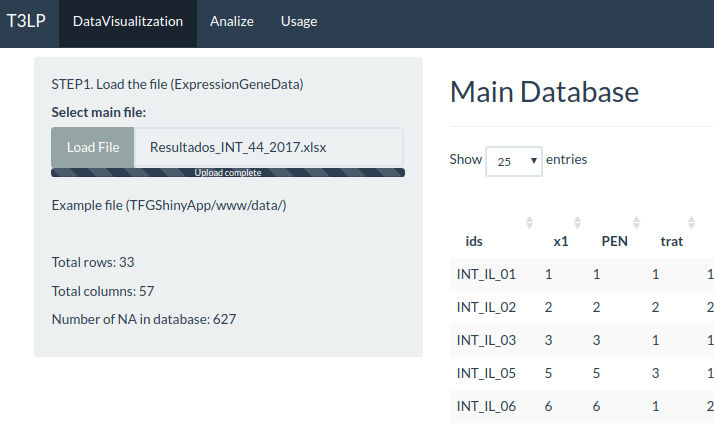
\includegraphics[scale=0.3]{app1.png}
\captionof{figure}{Imatge de l'aparen\c{c}a de l'aplicació i la seva estructura de pestanyes.}
\end{center}

La idea principal a l'hora de desenvolupar l'aplicatiu ha sigut la de crear un entorn atractiu i fàcil per a l'usuari. L'aplicació està formada de 3 pestanyes:
\begin{enumerate}
\item \textit{DataVisualitzation}: Pestanya on carreguem les dades i obtenim unes taules per poder fer consultes i visualitzar les dades.
\item \textit{Analize}: Aquesta pestanya conté la configuració dels paràmetres i, un cop executat, els resultats de l'anàlisi i algunes ajudes a la interpretació.
\item \textit{Usage}: Per últim, trobem les especificacions necessàries per obrir la base de dades i un petit tutorial de l'aplicatiu.
\end{enumerate}

\textbf{Observació}  Si existeixen problemes a l'hora d'obrir l'aplicació, a l'annex \ref{annex:d} podem trobar l'output de la funció \texttt{sessionInfo} on ens mostra la versió d'R utilitzada amb els corresponents paquets.
\clearpage
\subsection{Funcionalitats de l'aplicació}
En aquest apartat es presenten les funcionalitats que té l'aplicació en forma d'imatges i comentaris.
\\

\textbf{Observació.} Les dades utilitzades en les següents imatges no corresponen a les dades utilitzades en el cas d'estudi.
\subsubsection{Panell de configuració dels paràmetres}
També anomenat \textit{SidebarPanel}, en aquest panell trobem els paràmetres i variables relacionats amb l'estudi:
\begin{center}
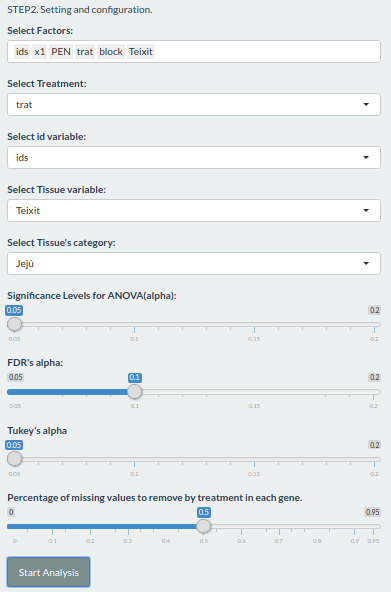
\includegraphics[scale=0.6]{app2.png}
\captionof{figure}{Panell de configuració dels paràmetres}
\end{center}
La configuració abans de comen\c{c}ar l'anàlisi està formada per:
\begin{enumerate}
\item Selecció dels factors de la base de dades.
\item Selecció de la variable tractament.
\item Selecció de la variable id.
\item Selecció de la variable teixit.
\item Selecció de la categoria de la variable teixit.
\item $\alpha$ per a l'ANOVA.
\item $\alpha$ BenjaminiHochberg(FDR).
\item $\alpha$ per a les comparacions 2 a 2 (Tukey).
\item Percentatge de dades faltants a eliminar per tractament per a cada gen (per defecte, el 50$\%$).
\end{enumerate}
\newpage
\subsubsection{Taules}
A l'aplicació podem trobar 2 taules de resultats, una corresponent a l'anàlisi de la variància i l'altre corresponent a les comparacions 2 a 2 dels tractaments.
\begin{center}
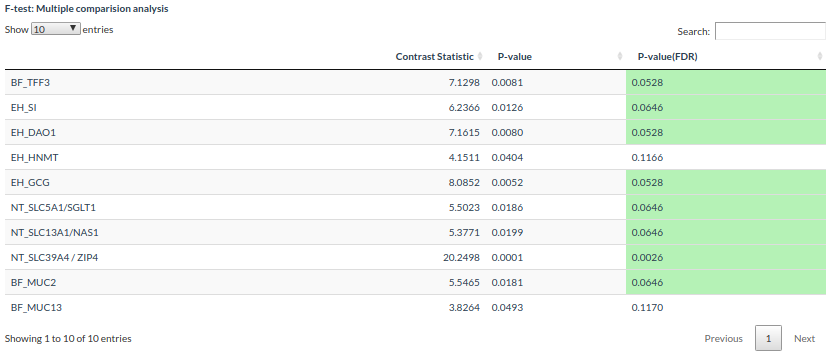
\includegraphics[scale=0.3]{app3.png}
\captionof{figure}{Taula de resultats de l'ANOVA}
\end{center}
\begin{center}
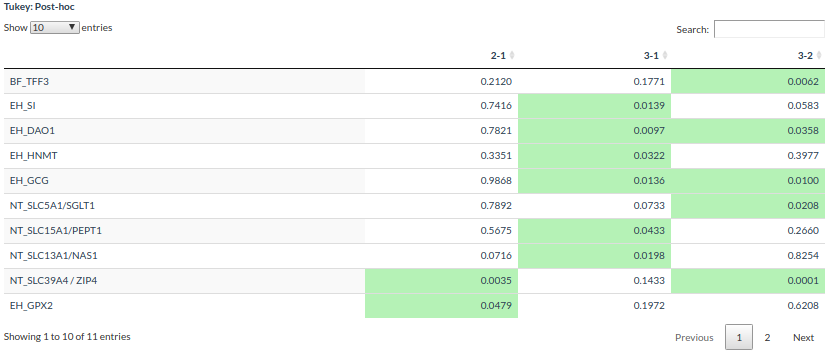
\includegraphics[scale=0.3]{app4.png}
\captionof{figure}{Taula de les comparacions 2 a 2 amb Tukey}
\end{center}
Les cel·les en verd mostren els p-valors que han sigut significatius. El nivell de significació s'estableix amb anterioritat per l'usuari al panell de configuració.
\subsubsection{Gràfics}
\noindent\textbf{LinePlot}\\

\noindent El primer gràfic que trobem correspon a les mitjanes per tractament i per gen. Aquest gràfic disposa de diferents opcions de personalització, com canviar l'ordre de les dades o fins i tot el color de les línies.
\begin{center}
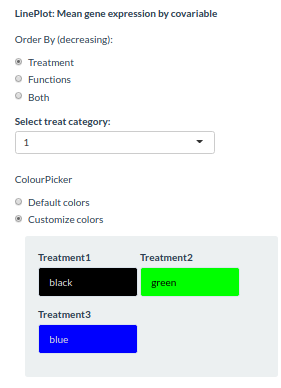
\includegraphics[scale=0.5]{app7.png}
\captionof{figure}{Panell de configuració del \textit{LinePlot}}
\end{center}
\clearpage
\begin{center}
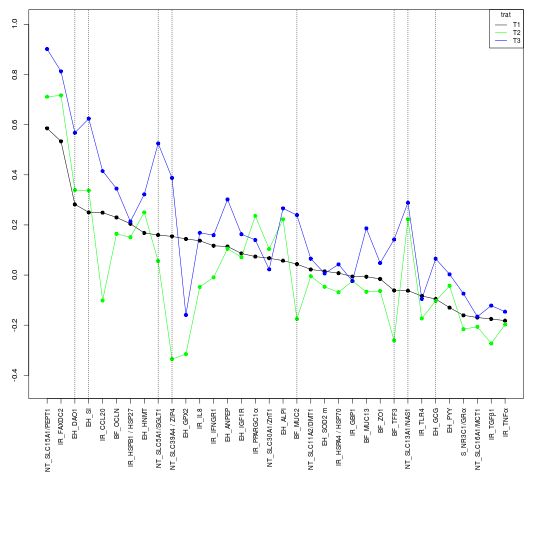
\includegraphics[scale=0.3]{app8.png}
\captionof{figure}{\textit{LinePlot}. Exemple on ordenem els gens (eix x) de forma decreixent pel valor del tractament 1 i escollim els colors per a cada tractament.}
\end{center}
\begin{center}
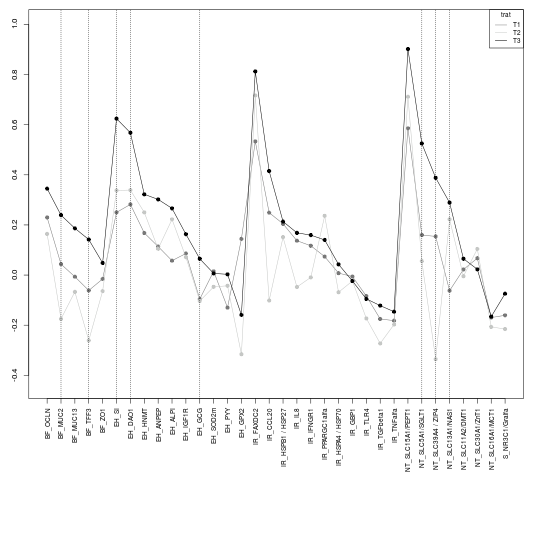
\includegraphics[scale=0.3]{app9.png}
\captionof{figure}{\textit{LinePlot}. Exemple on ordenem els gens (eix x) de forma decreixent pel valor del tractament 3 i agrupat per la funcionalitat del gen. A més escollim una escala de grisos.}
\end{center}
\newpage

\noindent\textbf{Representació gràfica de l'ACP}\\

\noindent Els gràfics de variabes i de casos s'interpreten conjuntament. La posició de les variables en el gràfic mostra l'estructura de les dades i suggereix possibles interpretacions de les components principals. Són gràfiques exploratòries, no porten significació estadística associada.\\

\noindent\textbf{Gràfic de variables}\\

\noindent Per a dades escalades o tipificades (cas habitual), les variables queden representades per fletxes de longitud entre 0 i 1. \\

\textbf{Longitud i qualitat de representació}. La longitud de la fletxa indica la mida de la seva projecció en el subespai de les components (preferentment, de les dues primeres) i, per tant, la seva  qualitat de representació: Una variable està  ben representada  en el subespai de les dues components, si la fletxa té longitud propera a 1, és a dir, s'aproxima a la circumferència de radi 1. (Només es poden interpretar les variables ben representades)\\

\textbf{Angles i correlació}. El cosinus de l'angle format pels dos vectors és proporcional a la seva correlació, per tant: \textit{Els angles que formen dues fletxes (o variables) entre sí, ens mostren la correlació existent entre les corresponents variables}. Els sentits dels vectors indiquen el signe de la correlació. L'angle que forma una fletxa (variable) i un eix (component) indica la correlació entre la variable i la component.\\

Per tant,\\
\begin{itemize}
\item Si dues variables estan ben representades, com més petit (proper a zero) sigui l'angle entre les seves fletxes, més forta i positiva és la seva correlació.

\item Si dues variables estan ben representades, com més  proper a 180$^o$ ($\pi$) sigui l'angle entre les seves fletxes, més forta i negativa és la seva correlació.

\item Si dues variables estan ben representades i l'angle entre les dues fletxes és proper al recte, la correlació és pràcticament zero.

\item Si hi ha un grup de variables ben representades i en posicions properes en el gràfic, això indica que totes elles estan molt relacionades entre sí i que ens subministren bàsicament la mateixa informació, diem que conformen \textit{un factor latent}.

\item Si apareixen varis grups de variables corrleacionades, vol dir que hi ha \textit{diversos factors latents} a la matriu de dades.

\item Si una o mès  variables estan ben representades i tenen un angle molt petit amb un dels eixos de coordenades, això indica que una de les components  està fortament correlacionada amb aquesta(es) variable(s) i, per tant, es pot interpretar (etiquetar) la component en base al significat d'aquesta(es) variable(s).
\end{itemize}

\noindent\textbf{Gràfic de casos individuals}\\

\noindent Els gens (en general, els casos) es representen mitjançant un diagrama de dispersió dels scores o puntuacions en l'espai de les components. Els casos amb puntuacions més elevades en una component es poden interpretar en base amb les variables més correlacionades amb aquesta component. Els colors de la gràfica de dispersió se solen utilitzar per visualitzar una variable qualitativa.
\begin{center}
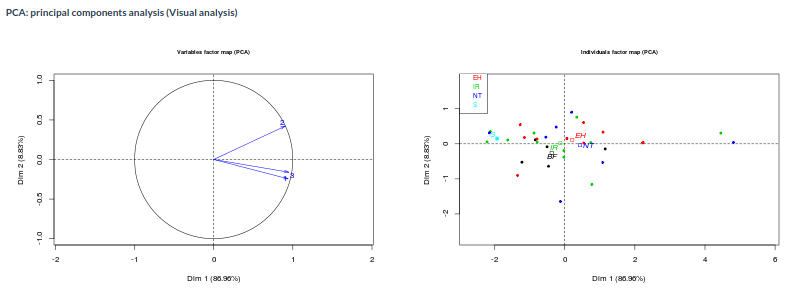
\includegraphics[scale=0.3]{app5.png}
\captionof{figure}{Representació gràfica de l'ACP}
\end{center}

\noindent\textbf{Heatmap}\\

\noindent El \textit{heatmap} és la respresentació conjunta de dos \textit{dendrogrames}: un dendrograma vertical que mostra agrupacions de files (gens o variables) i un dendrograma horitzontal que mostra agrupacions de columnes (mostres o casos). Un dendrograma és un arbre que representa una jerarquia de particions (des de la màxima on cada element és un clúster fins a la mínima on tots els elements estan agrupats en un clúster únic). Per decidir quina partició s'escull, un criteri és tallar l'arbre per on les \textit{branques són més llargues} (perquè correspon a maximitzar les distàncies entre els clústers resultants).
\begin{itemize}
\item Al dendrograma vertical hi ha els clústers dels gens. Després d'escollir la partició, els gens agrupats en un mateix clúster tendeixen a tenir pautes d'expressió similars en el conjunt de les mostres.
\item  La variable categòrica \textit{funció del gen} es visualitza segons els colors que veiem sota del dendrograma vertical, i és  útil per explorar si els gens agrupats en un mateix clúster (expressions similars) tendeixen a tenir la mateixa funcionlitat o, per contra, l'agrupació per clústers no es correspon a l'agrupacio per funcionalitats.
\item  Al dendrograma horitzontal hi ha els clústers de les mostres. Després d'escollir la partició, les mostres agrupades en un mateix clúster tendeixen a tenir pautes d'expressió similars en el conjunt dels gens.
\item  La variable \textit{tractament} es visualitza segons els colors que veiem sota del dendrograma horitzontal, i és útil per  explorar si les mostres d'un mateix clúster (expressions similars) tendeixen a correspondres a un mateix tractment o, per contra, l'agrupació per clústers no es correspon a l'agrupacio per tractaments.
\item  En blanc trobem els casos que són NA's.
\end{itemize}

\begin{center}
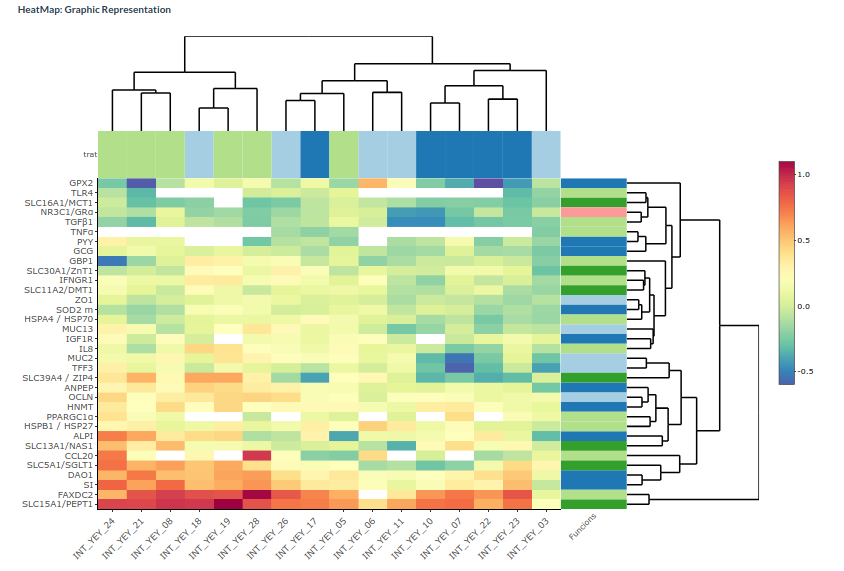
\includegraphics[scale=0.3]{app6.png}
\captionof{figure}{\textit{Heatmap} interactiu}
\end{center}

\subsection{Futures versions de l'aplicació}
A dia d'avui l'aplicació està a la versió 1.0.0. En aquest apartat es plantegen noves funcionalitats per a futures versions:
\begin{enumerate}
\item Utilitzar un servidor per tenir l'aplicatiu disponible en forma de pàgina web. D'aquesta manera es desvincula la necessitat que cada usuari compili l'aplicatiu des de el seu dispositiu. És una manera de facilitar als investigadors la feina, ja que no seria necessari tenir cap coneixement d'\texttt{R} per obrir l'aplicació.
\item La possibilitat de descarregar un informe, fet en \texttt{LateX}, dels resultats obtinguts.
\item Implementar métodes més acurats per a dissenys desbalancejats.
\item Implementar les gràfiques de barres d'error, per visualitzar les comparacions 2 a 2 (Tukey).
\item Fer encara més interactiva l'aplicació, amb nous gràfics de línies, si bé això podria anar en detriment del temps d'execució de l'anàlisi.
\end{enumerate}
Aquestes idees i altres que es puguin tenir, es poden implementar en un futur. El codi de l'aplicació és públic, i queda obert per a usuaris que vulguin col·laborar amb el projecte. L'únic necessari és registrar-se en la plataforma de \textit{GitHub} i sol·licitar una col·laboració a l'administrador del projecte.
\newpage
\section{Conclusions}
En aquest treball s'ha descrit un protocol d'anàlisi capa\c{c} d'analitzar i explorar diversos aspectes d'una base de dades d'expressió gènica d'un seguit de gens, on les mostres estan classificades segons un factor, habitualment un tractament, una dieta o una altra situació experimental...A més, analitzar les dades d'expressió gènica provinents de la tecnologia \textit{OpenArray} d'una manera senzilla i còmode per a l'usuari.
\\

La possibilitat d'utilitzar una eina específica per aquest tipus d'estudi, però que s'ha fet prou general i automàtica, obre un ventall de possibilitats als investigadors. La replicació de l'anàlisi amb futures dades és una realitat amb l'aplicatiu. A més la seva estructura interna facilita l'eventual integració de nous mètodes estadístics dins del codi. D'aquesta manera l'eina podria anar evolucionant al llarg del temps amb la finalitat de fer una anàlisi completa i apta per a altres dissenys.
\\

El treball de fi de grau m'ha permès aprofundir en temes bàsics de la inferència estadística (ANOVA, Tukey) i de l'anàlisi multivariant (PCA, anàlisi de clústers), entre altres. Al mateix temps, he estudiat conceptes o recursos que no havia tractat durant el grau (FDR, heatmap), dels quals he fet recerca bibliogràfica. També he pogut practicar i ampliar elements de programació (\texttt{R},\texttt{Shiny}, gestió de versions, etc.,), alguns dels quals he après de manera autodidacta. Finalment, voldria destacar el caràcter multidisciplinar d'aquest treball, entre estadística, biomedicina i bioinformàtica, que suposa un nexe d'unió entre algunes assignatures que he cursat durant el grau.
\section{Agraïments}
\label{agr}
Per portar endavant aquest projecte he necessitat l'ajuda d'algunes persones a les quals volia agrair la seva col·laboració i esfor\c{c}.\\

Agrair la col·laboració de l'estudiant de veterinària Francesc Gonzàlez i el Dr. David Solà.\\

També voldria donar les gràcies a la tutora del treball, la Dr. Mercè Farré, per guiar-me durant el projecte i posar la seva confian\c{c}a en mi.
%Bibliografia
\clearpage
\begin{thebibliography}{aaaa}
\bibitem{tami}
Guillermo Ayala.(2018).Bioinformática Estadística: Análisis estadístico de datos ómicos. \pageref{1.1}
\\\texttt{https://www.uv.es/ayala/docencia/tami/tami13.pdf}
\bibitem{effron}
Efron, B., $\&$ Hastie, T. (2016). Computer Age Statistical Inference: Algorithms, Evidence, and Data Science (Institute of Mathematical Statistics Monographs). Cambridge: Cambridge University Press. pp. 271-294, doi:10.1017/CBO9781316576533. \pageref{2.2}
\bibitem{multi}
Everitt, B., Hothorn, T. : An introduction to Applied Multivariate Analysis with R. Springer. 2011. \pageref{2.4}
\bibitem{multi2}
Härdle, W., Simar, L.: Applied Multivariate Statistical Analysis. Springer. 2007. \pageref{2.4}
\bibitem{fdr}
Controlling the False Discovery Rate: A Practical and Powerful Approach to Multiple Testing Journal of the Royal Statistical Society. Series B (Methodological), Vol. 57, No. 1. (1995), pp. 289-300, doi:10.2307/2346101 by Yoav Benjamini, Yosef Hochberg. \pageref{2.2.1}

\bibitem{cite2}
Ramón Tamarit Agusti. Análisis de cluster no supervisados. Aplicaciones en
la búsqueda y visualización de perfiles de expresión
en datos de microarrays. \pageref{2.4.1}
\\\texttt{http://mural.uv.es/rata3/PECSspace.html}

\bibitem{cite3}
Dong Hyun Jeong, Caroline Ziemkiewicz, William Ribarsky and Remco Chang: Understanding Principal Component Analysis Using a Visual Analytics Tool. \pageref{2.4.3}
\\\texttt{http://www.knowledgeviz.com/pdf/UKC2009.pdf}

\bibitem{cite5}
Universidad de Granada: Métodos de análisis multivariante. Análisis clúster. \pageref{2.4.1}
\\\texttt{http://wpd.ugr.es/$\sim$bioestad/guia-spss/}

\bibitem{cite6}
Universidad de Granada: Métodos Jerárquicos de Análisis Cluster. \pageref{2.4.1}
\\\texttt{http://www.ugr.es/$\sim$gallardo/pdf/cluster-3.pdf}

\bibitem{cite7}
\textit{NCBI, National Center of Biotechnology Information.}
\\\texttt{https://www.ncbi.nlm.nih.gov/}. USA

\bibitem{cite8}
\textit{PubMed. US National Library of Medicine.}
\\\texttt{https://www.ncbi.nlm.nih.gov/pubmed/}. USA

\end{thebibliography}
%%Appendix
\clearpage
\appendix
\onecolumn
\section{Mètode de Ward: Exemple del mètode amb gens}
\label{annex:a}
Observem com funciona aquest mètode en el cas de tenir 3 gens on es mesura l'expressió gènica per a 3 mostres. Les dades són les següents:
\begin{table}[ht]
\centering
\begin{tabular}{rrrr}
\hline
& $X_{1}$ & $X_2$ & $X_3$ \\
\hline
$Gen_1$ & 1.02 & 0.21 & 6.29 \\
$Gen_2$ & 10.06 & 8.19 & 7.29 \\
$Gen_3$ & 10.11 & 14.63 & 7.62 \\
\hline
\end{tabular}
\caption{Expressió gènica de cada gen $Gen_i$ per a cada mostra $X_j$.}
\end{table}
\\
Recordem que per utilitzar aquest mètode necessitem la matriu de distàncies euclidianes. La distància euclidiana entre dos punts ${\displaystyle \,P=(p_{1},p_{2},\dots p_{n})}$ i $ {\displaystyle \,Q=(q_{1},q_{2},\dots q_{n})}$ es defineix com:
\begin{equation*}
{\displaystyle d_{E}(P,Q)={\sqrt {(p_{1}-q_{1})^{2}+(p_{2}-q_{2})^{2}+\cdots +(p_{n}-q_{n})^{2}}}}
\end{equation*}
Per tant, obtenim aquesta matriu de distàncies:
\begin{table}[ht]
\centering
\begin{tabular}{rrrr}
\hline
& $Gen_1$ & $Gen_2$ & $Gen_3$ \\
\hline
$Gen_1$ & 0 & 12.10 & 17.10 \\
$Gen_2$ & 12.10 & 0 & 6.45 \\
$Gen_3$ & 17.10 & 6.45 & 0 \\
\hline
\end{tabular}
\caption{Matriu de distàncies. La distància utilitzada és l'euclidiana.}
\end{table}
\\
En aquest cas, com tenim només 3 gens, tenim un total de 3 combinacions possibles de 2 elements. Per tant, calcularem $\bigtriangleup E$ per a cada combinació i escollirem el més petit com el millor clúster.
\\

\begin{table}[ht]
\onecolumn
\centering
\begin{tabularx}{\linewidth}{llllll}
\hline
& $Particions$ & $Centroides$ & $E_k$ & $E$ & $\bigtriangleup E$ \\
\hline
& $(Gen_1,Gen_2),Gen_3$ & $C_{Gen_1,Gen_2} = (5.54,4.19,6.78) $ & $E_{Gen_1,Gen_2}=72.92$
$E_{Gen_3}=0$ & $72.92$ & $72.92$ \\
& $(Gen_1,Gen_3),Gen_2$ & $C_{Gen_1,Gen_2} = (7.06,7.67,7.06) $ & $E_{Gen_1,Gen_3}=112.42$
$E_{Gen_2}=0$ & $112.42$ & $112.42$ \\
& $(Gen_2,Gen_3),Gen_1$ & $C_{Gen_1,Gen_2} = (10.08,11.41,7.45)$ & $E_{Gen_2,Gen_3}=41.5850$
$E_{Gen_1}=0$ & $41.5850$ & $41.58$ \\
\hline
\end{tabularx}
\caption{Taula resum dels càlculs proposats per obtenir l'increment de la suma de quadrats residuals. Les particions són possibles combinacions de 2 gens en un total de 3.}
\end{table}

\noindent Podem observar que segons el criteri de Ward, escolliríem unificar el $Gen_2$ i el $Gen_3$ en un mateix clúster. Si fem el mateix però automàticament amb la funció \texttt{hclust}, obtenim el següent dendrograma:
\begin{center}
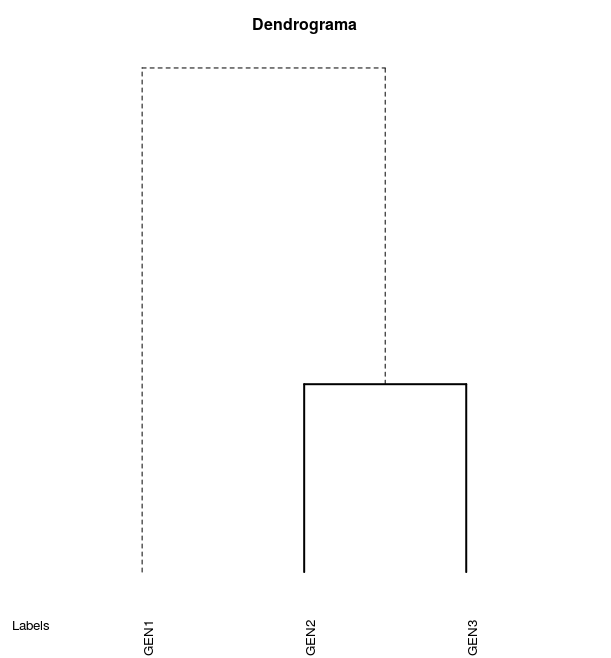
\includegraphics[scale=0.4]{dendrograma.png}
\captionof{figure}{Dendrograma obtingut amb la funció \texttt{hclust}. Si apliquem directament la funció \texttt{hclust}, que utilitza el mètode de Ward, obtenim 2 clústers. El primer clúster amb el $Gen_1$ i un segon clúster amb el $Gen_2$ i el $Gen_3$. Trobem els mateixos clústers amb el procediment manual que hem calculat anteriorment. L'altura a la qual s'uneixen els clústers és $\bigtriangleup E$, en aquest cas, el $Gen_2$ i el $Gen_3$ s'uneixen a una altura de $41.58$.}
\end{center}
\section{Gens diana utilitzats a l'estudi}
\label{annex:b}
\begin{center}
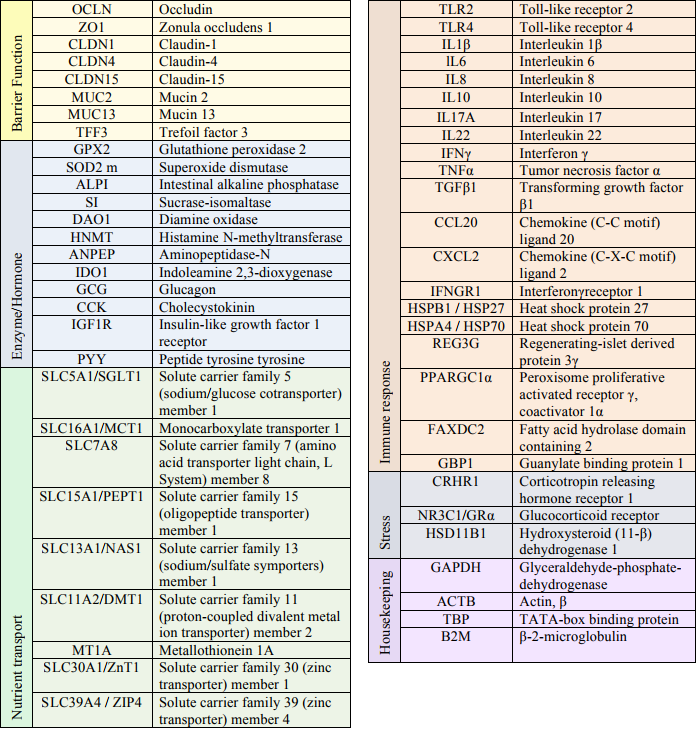
\includegraphics[scale=0.7]{genes.png}
\captionof{figure}{Gens \textit{diana} i la seva funció dins de l'organisme.}
\end{center}
\clearpage
\section{Output sessionInfo()}
\label{annex:d}
\lstinputlisting[float=ht,frame=tb,caption=Output sessionInfo(),label=zebra]{output.txt}
\end{document}
\grid
